%%%%%%%%%%%%%%%%%%%
%% imports
%%%%%%%%%%%%%%%%%%%
\documentclass[12pt,twoside,a4paper,parskip]{scrbook} % oneside for writing, twoside for submission (space for comments on the print)
\setcounter{tocdepth}{1} % depth of table of contents, for debugging purposes
\usepackage[utf8]{inputenc} % define the encoding type for LateX, may be obsolete in newer versions of LateX
\usepackage{csquotes} % helper package for quotes
\usepackage[english]{babel} % language support, multiple languages can also be listed
\usepackage{floatflt} % wrap text around tables and figures, useful for some templates
\usepackage[pdftex]{graphicx} % /includegraphics command with more options
\usepackage[hidelinks]{hyperref} % used for cross-referencing in LateX, hidelinks is an option to better format links
\usepackage{xcolor} % color management
\usepackage{amssymb} % symbol support
\usepackage{textcomp} % text symbol support
\usepackage{nicefrac} % better formatting for fractions
\usepackage{scrhack} % definition of macros 
\usepackage{pdfpages} % include pdf pages in LaTeX
\usepackage{float} % floating objects (i.e. figures, tables)
\usepackage{pdflscape} % better pdf support with more options
\usepackage[verbose]{placeins} % checks that floats are within bounds - verbose adds extra logs
\usepackage[markcase=ignoreuppercase,headsepline,plainfootsepline]{scrlayer-scrpage} % manage page styles, markcase: automatic typesetting in heads, headsepline: line underneath the headerm, plainfootsepline: rule above the footer
\usepackage[ruled,vlined]{algorithm2e} % algorithm environment, ruled: algorithm with line at the top and bottom. Caption is not centered but at the beginning of the algorithm, vlined: vertical line followed by a small horizontal line between the start and the end of each block
\usepackage{listings} % used to display nicely formatted source code 
\usepackage{caption} % adds captions to figures, tables, equations... with correct number assignments
\usepackage{subcaption} % adds subcaptions to subfigures, useful for more complex figures, has to be imported after the caption package
\usepackage{epstopdf} % needed to use .eps 
\usepackage{longtable} % enables long tables over page boundaries
\usepackage{setspace} % sets line spacing
\usepackage{booktabs} % better line management and line separation within tables
\usepackage[sortcites,style=numeric,backend=biber,doi=false,isbn=false,eprint=false]{biblatex} % good package for bibliography support in LaTeX with biber backend, sortcites: sorting bibliography (name, title, year), style=numeric: standard numeric citation style (recommended!), doi/isbn/url/eprint=false: hide links in bibliography (recommended for clean bibliography!)
\usepackage{makecell} % tabular column heads and multilined cells
\usepackage{amsmath} % math support 
\bibliography{literatur.bib} % included biblatex formatted citations from the file bibliography.bib
\usepackage{algorithmic}
\usepackage{multirow}
\usepackage{multicol}
\usepackage{pifont}
\usepackage{lipsum} % only used for the template generation, remove this usepackage command and all \lipsum calls
\usepackage{graphicx} % Required for inserting images
\usepackage{enumitem}
\usepackage[hypcap=true]{caption}
%%%%%%%%%%%%%%%%%%%
%% definitions
%%%%%%%%%%%%%%%%%%%
\def\BaAuthor{Mahesh Saravanan \\ K54723}
\def\BaAuthorStudyProgram{Master of Artificial Intelligence} 
\def\BaType{Master Thesis}
\def\BaTitle{Simulation Environments and AI-based Autonomous Driving Solutions - a Comparative Evaluation}
\def\BaSupervisorOne{Prof. Dr. Christian Bachmeir}
\def\BaSupervisorTwo{Mr. Leon Heller}
\def\BaDeadline{\SubmitDate}
\def\SubmitDate{18.01.2023}
\def\git{https://github.com/Mahesh-Saravanan/}

% option to generate anonymous submission for plagiarism scan!
\ifdefined\iswithfullname
\def\ShowBaAuthor{\BaAuthor}
\else
\def\ShowBaAuthor{N.~N.}
\fi

\hypersetup{
pdfauthor={\ShowBaAuthor},
pdftitle={\BaTitle},
pdfsubject={Subject},
pdfkeywords={Keywords}
}

%%%%%%%%%%%%%%%%%%%
%% configs to include
%%%%%%%%%%%%%%%%%%%
\colorlet{punct}{red!60!black}
\definecolor{background}{HTML}{EEEEEE}
\definecolor{delim}{RGB}{20,105,176}
\colorlet{numb}{magenta!60!black}

\definecolor{gray}{rgb}{0.4,0.4,0.4}
\definecolor{darkblue}{rgb}{0.0,0.0,0.6}
\definecolor{cyan}{rgb}{0.0,0.6,0.6}

\definecolor{pblue}{rgb}{0.13,0.13,1}
\definecolor{pgreen}{rgb}{0,0.5,0}
\definecolor{pred}{rgb}{0.9,0,0}
\definecolor{pgrey}{rgb}{0.46,0.45,0.48}

\lstset{
  basicstyle=\ttfamily,
  columns=fullflexible,
  showstringspaces=false,
  commentstyle=\color{gray}\upshape
  linewidth=\textwidth
}

\lstdefinelanguage{json}{
    basicstyle=\normalfont\ttfamily,
    numbers=left,
    numberstyle=\scriptsize,
    stepnumber=1,
    numbersep=8pt,
    showstringspaces=false,
    breaklines=true,
    backgroundcolor=\color{background},
    literate=
     *{0}{{{\color{numb}0}}}{1}
      {1}{{{\color{numb}1}}}{1}
      {2}{{{\color{numb}2}}}{1}
      {3}{{{\color{numb}3}}}{1}
      {4}{{{\color{numb}4}}}{1}
      {5}{{{\color{numb}5}}}{1}
      {6}{{{\color{numb}6}}}{1}
      {7}{{{\color{numb}7}}}{1}
      {8}{{{\color{numb}8}}}{1}
      {9}{{{\color{numb}9}}}{1}
      {:}{{{\color{punct}{:}}}}{1}
      {,}{{{\color{punct}{,}}}}{1}
      {\{}{{{\color{delim}{\{}}}}{1}
      {\}}{{{\color{delim}{\}}}}}{1}
      {[}{{{\color{delim}{[}}}}{1}
      {]}{{{\color{delim}{]}}}}{1},
}

\lstset{language=xml,
  morestring=[b]",
  morestring=[s]{>}{<},
  morecomment=[s]{<?}{?>},
  stringstyle=\color{black},
  numbers=left,
  numberstyle=\scriptsize,
  stepnumber=1,
  numbersep=8pt,
  identifierstyle=\color{darkblue},
  keywordstyle=\color{cyan},
  backgroundcolor=\color{background},
  morekeywords={xmlns,version,type}% list your attributes here
}

\lstset{language=Java,
  showspaces=false,
  showtabs=false,
  tabsize=4,
  breaklines=true,
  keepspaces=true,
  numbers=left,
  numberstyle=\scriptsize,
  stepnumber=1,
  numbersep=8pt,
  showstringspaces=false,
  breakatwhitespace=true,
  commentstyle=\color{pgreen},
  keywordstyle=\color{pblue},
  stringstyle=\color{pred},
  basicstyle=\ttfamily,
  backgroundcolor=\color{background},
%  moredelim=[il][\textcolor{pgrey}]{$$},
%  moredelim=[is][\textcolor{pgrey}]{\%\%}{\%\%}
}
\newcommand*{\forcetwoside}[1][1]{%
 \begingroup
   \cleardoubleoddpage
   \KOMAoptions{titlepage=true}% useful e.g. for scrartcl
   \csname @twosidetrue\endcsname
   \maketitle[{#1}]
 \endgroup
}
\def\c#1{\mathcal{#1}}
\DeclareUnicodeCharacter{2212}{-}
\setcounter{tocdepth}{2}
\setcounter{secnumdepth}{5}


\renewcommand\theparagraph{\arabic{section}.\arabic{subsection}.\arabic{subsubsection}.\alph{paragraph}}

\begin{document}
%%%%%%%%%%%%%%%%%%%
%% Title page
%%%%%%%%%%%%%%%%%%%
\ifdefined\print
\newgeometry{centering}    %%% make the page centered on paper
\begin{titlepage}
	\newcommand{\HRule}{\rule{\linewidth}{0.5mm}}
	\centering
	\begin{center}
		\vspace*{.06\textheight}	
		\HRule \\[0.4cm] % Horizontal line
		{\huge \bfseries \BaTitle \par}\vspace{0.4cm} % Thesis title
		\HRule \\[1.5cm] % Horizontal line
		\vspace{4.5cm}
		\begin{minipage}[t]{0.4\textwidth}

		\centering
		{\large \BaAuthor} 

		\end{minipage}
		\vfill
		\vspace*{.1\textheight}
		{\large \BaType}\\[0.5cm] % Thesis type
		{\large University of Applied Sciences Würzburg-Schweinfurt}\\[0.5cm]
		{\large \SubmitDate}\\[4cm] % Date
		\vfill
	\end{center}
\end{titlepage}
\restoregeometry
\fi
\frontmatter
\titlehead{%  {\centering side head}
  {Technical University of Applied Sciences Würzburg-Schweinfurt (THWS)\\
   Faculty of Computer Science and Business Information Systems\\\\
	}}
\subject{\BaType}
\title{\BaTitle\\[15mm]}
\subtitle{\normalsize{submitted to the Technical University of Applied Sciences W\"{u}rzburg-Schweinfurt in the Faculty of Computer Science and Business Information Systems to complete a course of studies in \BaAuthorStudyProgram}}
\author{\ShowBaAuthor}
\date{\normalsize{Submitted on: \BaDeadline}}
\publishers{
  \normalsize{Initial examiner: \BaSupervisorOne}\\
  \normalsize{Secondary examiner: \BaSupervisorTwo}\\
}
\lowertitleback{
\centering
\includegraphics[width=4cm]{Images/qrcode-thesis.png}
}
\forcetwoside



%%%%%%%%%%%%%%%%%%%
%% abstract
%%%%%%%%%%%%%%%%%%%

\section*{Abstract}
This thesis presents a comprehensive approach to evaluate and enhance autonomous vehicle simulators. The research comprises two primary works. Firstly, a systematic evaluation methodology is introduced, establishing a scoring system based on 73 discerning parameters to assist users in efficiently selecting a suitable simulator. This method streamlines the process, enabling users to assess simulator capability aligned with their specific needs.

Secondly, the thesis explores the development of a prototype simulator driven by a deep generative model. This model aims to simulate the transition of 2D lidar data and generate diverse scenarios crucial for training machine learning models in autonomous driving. 

The study assesses the performance of the system of comparison by evaluating existing simulators and user preferences and discusses the performance of the proposed prototype simulator.


\section*{Zusammenfassung}
Zusammenfassung
In dieser Arbeit wird ein umfassender Ansatz zur Bewertung und Verbesserung von Simulatoren für autonome Fahrzeuge vorgestellt. Die Forschungsarbeit besteht aus zwei Hauptteilen. Erstens wird eine systematische Bewertungsmethodik eingeführt, die ein Punktesystem basierend auf 73 unterscheidbaren Parametern entwickelt, um Benutzer bei der effizienten Auswahl eines geeigneten Simulators zu unterstützen. Diese Methode vereinfacht den Prozess und ermöglicht es den Benutzern, die Fähigkeiten des Simulators entsprechend ihrer spezifischen Bedürfnisse zu bewerten.

Zweitens wird in dieser Arbeit die Entwicklung eines Prototyps eines Simulators untersucht, der durch ein tiefes generatives Modell gesteuert wird. Dieses Modell zielt darauf ab, den Übergang von 2D-Lidar-Daten zu simulieren und verschiedene Szenarien zu generieren, die für das Training maschineller Lernmodelle für das autonome Fahren entscheidend sind. 

Die Studie evaluiert die Leistung des Referenzsystems durch die Bewertung bestehender Simulatoren und Benutzerpräferenzen und diskutiert die Leistung des vorgeschlagenen Prototypsimulators.

% cSpell:disable


\newpage
\chapter*{Acknowledgment}
I would like to thank Prof. Dr. Christian Bachmeir from Technical University of applied sciences Würzburg Schweinfurt for providing me an opportunity to work on this topic and for his supervision throughout this endeavour.

I would also like to thank Mr. Leon Heller for his unwavering support, continuous guidance, and supervision throughout the course of this thesis. His invaluable ideas and insights significantly contributed to shaping this work.

I am also thankful to the other professors whose contributions fine-tuned and catalysed this research through their knowledge and feedback. Additionally, I express my appreciation to my family and friends for their support throughout this journey.

%%%%%%%%%%%%%%%%%%%
%% toc
%%%%%%%%%%%%%%%%%%%
\tableofcontents
%%%%%%%%%%%%%%%%%%%
%% Main part of the thesis
%%%%%%%%%%%%%%%%%%%
\mainmatter

\chapter{Introduction}\label{ch:intro}
\section{Autonomous Vehicles}
Transportation has played an important role in the human history, evolving from the invention of the rotary wheel to the modern road cars. The invention of fuel engines in the last century marked a significant revolution, impacting faster goods transportation and extending to civilian life with the introduction of road cars. This period also witnessed the development of proper road infrastructures to accommodate the advancements in vehicle performance. The fourth industrial revolution mark a start of new era where intelligent systems-controlled machines are developed which reduces the manual errors and enhancing performance. The automotive industry is also undergone this transformation with various intelligent driver assistance systems like Advanced Driver Assistance Systems (ADAS) which not only reducing human effort in driving but also ensuring safety. Engineers and scientists globally are working to enhance the capabilities of intelligent systems, aiming for complete autonomous driving, eliminating the need for human guidance. 

The concept of autonomous driving dates back to 1926, with the development of a radio-controlled car in New York City. In 1960s, the Transport and Road Research Laboratory in the United Kingdom laid magnetic cables beneath the road, serving as a path detection tool for self-driving cars and tested its performance. Later, in 1995 Mercedes Benz achieved a significant milestone with the development of first self-sufficient autonomous vehicle, a retrofitted Mercedes S class equipped with efficient cameras and exclusive processors for parallel computing. This vehicle reached a maximum speed of 175 kmph, covering 1500 kms from Munich, Germany, to Copenhagen, Denmark, performing various manoeuvres in traffic without human assistance. In the late 2000s, carmakers like Toyota and Volvo, along with tech companies such as Google and Waymo, developed their prototypes of Autonomous Vehicles (AVs). 
The parallel advancements in the field of Artificial Intelligence and efficient hardware accelerated research in self-driving technology. Notably, improvements in cameras and GPUs facilitated fast and efficient processing, while intelligent algorithms like neural networks laid the foundation for Autonomous Vehicles (AVs). In 2014, Tesla Motors launched Model S, a semi-autonomous driving car. This vehicle featured a various assistance feature, including lane detection, autonomous braking and parking, and speed limit recognition using computer vision. Tesla's entry into functional semi-autonomous driving represented a notable advancement in the field. During the same year, the Society of Automotive Engineers (SAE) had drafted a 6-level taxonomy for autonomous driving. This framework provided a standardized and structured classification system for assessing the level of autonomy in vehicles. Recognizing the growing impact of autonomous driving, several countries, including the United States of America, the United Kingdom, and Japan, made decisions to formulate laws addressing autonomous driving in the next few years. Various leading car manufacturers, including Mercedes Benz, BMW, and Volvo, have introduced their commercial fully or semi-autonomous production vehicles. They are continually enhancing their automation levels, as classified by the Society of Automotive Engineers (SAE). For instance, in 2022, Mercedes Benz achieved SAE Level 3 automation with its S-Class and EQS models, equipped with advanced driving technologies like an automated lane-keeping system. However, Tesla Motors has been a leader in this field, showcasing superior performance.
The SAE J3016 classifies autonomous vehicles into six levels, ranging from fully manual driving to fully automated systems as described in Table \ref{tab:automation-levels} \cite{sae2019}

\begin{table}[htbp]
  \centering
  
  \begin{minipage}{\linewidth}
    \renewcommand{\arraystretch}{1.3} 
    \begin{tabular}{|c|c|p{8cm}|}
      \hline
      \textbf{Level} & \textbf{Name} & \textbf{Description} \\
      \hline
      0 & No driving automation & This level involves no driving assistance system, and the entire driving process is manually controlled. \\
      \hline
      1 & Driver assistance & Vehicles at this level feature a single automated system under the driver's supervision. \\
      \hline
      2 & Partial driving automation & Multiple automated systems, such as automated steering and braking, work simultaneously under the driver's attention. The driver must be ready to take control at any moment. \\
      \hline
      3 & Conditional driving automation & This level involves a system with an intelligent algorithm capable of making decisions like overtaking navigation. However, human attention is still required. \\
      \hline
      4 & High driving automation & At this level, the vehicle can make optimistic decisions in the event of a failure, reducing the need for human interaction. This level is often suitable for confined areas or regions. \\
      \hline
      5 & Full driving automation & Here, the vehicle can perform all driving tasks without human interaction, comparable to an experienced human driver. \\
      \hline
    \end{tabular}
  \end{minipage}
  \caption{Levels of Driving Automation}
  \label{tab:automation-levels}
\end{table}

Driver-less vehicles find applications not only in passenger cars but also across various areas like shuttling people on campuses, moving goods in warehouses, and in military operations. Especially in industries, these automated machines could transport goods across the premises which save time and minimize human error. However, ensuring their safety of operation is crucial especially when it comes to road cars. Governments worldwide are creating regulations for autonomous mobility. Moreover, vehicle manufacturers are enhancing hardware and software while conducting extensive testing to ensure safety and prevent failures.
\section{Simulators}
Simulators imitate real-world systems, replicating their dynamics and features. They come in different types: software, hardware, or a mix of both. These systems replicate various functions, interacting with users, taking inputs, and providing feedback to the users. For example, driving simulators create visual environments and hardware setup for driver training and testing, Which takes control commands from users and update their states. Simulators can be classified based on various features Some of the examples are
%\paragraph{Based on Time}
\paragraph*{Discrete Event Simulation:}
Each step happens at distinct intervals, which are mapped to specific durations. Driving simulators fall into this category, where observation states change at each step. The time duration of a single time step is defined by required precision.
\paragraph*{Continuous Simulation:} In this type of simulation, time moves continuously without distinct steps, backed by differential equations. These are useful for modelling continuous events like microbe growth in biology.
\paragraph*{Stochastic Simulation:}
This type of simulation introduces a controlled amount of randomness within sensible limits in the parameters. It's helpful for studying systems with random noise, like analysing daily usage patterns on a social media site.
\paragraph*{Deterministic Simulation:}
These systems operate using deterministic algorithms without any randomness. They're commonly applied in engineering. The outcomes of these simulations remain consistent and reproducible for a specific set of parameters.
\paragraph*{HiL simulation:} Hardware-in-the-Loop (HiL), is a testing method integrating physical hardware components into a simulated environment. In HIL setups, real hardware, like sensors and control systems, connects to a computerized simulation. This allows the actual hardware to interact with a virtual environment, enabling thorough testing of systems under various scenarios. In Autonomous vehicle development, car sensors and control units are connected to a simulated driving scenario, allowing engineers to assess how the physical components respond to different conditions before deploying them in real-world situations. HIL testing ensures more robust and validated performance of hardware and systems in a controlled, simulated environment before practical implementation.

Users can tweak these parameters to test and tune the results of the system. Usually, simulations help to find the optimal parameters and it have diverse applications, for events spanning millions of years to nanoseconds. Simulations play a vital role in result analysis, safety engineering, and design processes. They save significant time during testing and can enhance the testing outcomes. For instance, testing the driving of an autonomous car for 10,000 km in the real world demands a lot of time and resources, whereas using a simulator significantly reduces this time-frame. However, there's often a discrepancy between the real world and simulations, which might lead to errors in analysis. In fields like machine learning and robotics, it contributes a crucial role. One of the three paradigm of Machine learning is reinforcement learning where a virtual agent within a simulator takes diverse actions under various conditions and learns from the feedback provided. In robotics, algorithm which drives the robots are trained using simulation for tasks like localization, pick and place, faulty detection…
\section{Problem Statement}
\subsection{Lack of system of comparison}
In the growing domain of autonomous vehicle research, simulator plays a significant role in the process of development such as algorithm training, performance evaluation across diverse environments and comparison of method. There are numerous simulators, varying in types and functionalities, available in the community for direct or indirect use in research works. In addition, the domain of self-driving vehicle research itself is broad, includes distinct applications such as indoor robots, industrial autonomous vehicles (AVs), on-road vehicles, and semi-autonomous vehicles. Each application requires a unique simulator tailored to its specific requirements.

The challenge arises due to the diversity among these simulators and their requirements, each comes with its own set of advantages, features, and limitations. Consequently, comparing and selecting the most suitable simulator becomes a complex task. For instance, a simulator might perform well in numerous aspects, yet fail to simulate a crucial sensor required by a user, making it unsuitable for that specific application. Conversely, another simulator might lack certain features but could be better suited for the user. 

The aim of this thesis is to establish a concrete set of metrics for comparison purposes. The proposed metric will be generic and adaptable to individual user preferences. Users will have the flexibility to adjust the importance of criteria based on their requirements and they are universally applicable across all types of autonomous vehicle simulators. Through this systematic approach, users could able to assign personalized ratings to simulators, facilitating informed decision-making in selecting the most suitable simulator according to their preferences and needs.

\subsection{Simulator based on Generative AI}
Generative AI had gained momentum in recent years, continuously improving its performance. This field primarily uses deep neural networks, trained on any provided data, learning its distribution. These trained models can generate novel, meaningful data samples which are not present in the training set but similar to it. 

In the domain of autonomous vehicle simulators, rendering new scenarios and environments is a one of its objectives. This feature enhances its suitability for algorithm testing across diverse environments, potentially improving the model’s performance. It’s also important that these new scenarios closely resemble real-world features while being meaningful and plausible.

Sensors in Autonomous cars play a important role in understanding the real world where the vehicle navigates. These vehicles utilize data from various of sensors such as cameras, Lidar, and radar to perceive their surroundings. The second part of this thesis aims to design and develop a simulator driven by a Generative AI model trained on real-world sensory data. The expected outcome is the generation of new, meaningful sensory data can effectively represent diverse and realistic environments. The simulator will operate on discrete time steps, ensuring that the generated data remains relative to preceding time steps.

\section{Structure of the thesis}
The thesis structure is as follows: Chapter 2, the Literature Review, is divided into three parts. The first segment analyses feature of popular autonomous vehicle simulators, followed by the discussion of existing comparative metrics for these simulators. The final part explores some of the relevant GAN architectures. Chapter 3 outlines the proposed method for comparing AV simulators, while Chapter 4 details the idea of Generative Model-based Simulator. Chapter 5 presents and discusses results, followed by the Conclusion and possible future works in this thesis.

\chapter{Literature Review}
This chapter explores different works related to the topic. The initial section examines the existing state-of-the-art autonomous vehicle simulators. The second part provides a summary of previous methodologies used to define a comparative metric for evaluating autonomous vehicle simulators. The last part of this chapter discusses about the different types of Generative Adversarial networks (GANs), a type of Generative AI algorithm utilized in this thesis. 
\section{State-of-art-Simulators}
Numerous simulators are available in the market, but this section analyse some relevant and popular simulators and highlighting their advantages, limitations and applications.
\subsection{CARLA}
CARLA, (Car Learning to Act) is an open-source software developed collaboratively by the Computer Vision Centre (CVC) and the Barcelona Super computing Centre (BSC) in partnership with the Toyota Research Institute. It is primarily designed for autonomous driving research and development, which features diverse and realistic environments, various climates and wide range of sensors. CARLA operates on a server-client architecture, built on Unreal Engine 4 and utilizing the OpenDRIVE standard 1.4 to define roads and urban settings. This unique structure allows the server to manage physics of simulator and computation while enabling user to communicate the server through C++ and Python APIs, providing scalability.

A notable feature of CARLA is its seamless support for developing, training, and validating machine learning algorithms. Researchers had experimented various algorithms like modular pipelines, imitation learning, and reinforcement learning within this simulator \cite{Carla}. Leveraging Unreal Engine 4, CARLA offers high-quality, realistic rendering of environments. Figure \ref{fig:CARLA} \cite{Carla} showcases scenes from the simulator in different weather conditions. Additionally, it supports an array of built in sensors such as camera, LiDAR and provides the user with various metadata, and ground truth. Moreover, CARLA offers access to diverse digital assets (actors, buildings) within the environment, meticulously designed to maintain a high level of realism \cite{Carla}. However, it currently offers support for only two pre-defined urban maps covering 2.9 km and 1.4 km, which limits its diversity and generalization capabilities.

\begin{figure}[h]
    \centering
    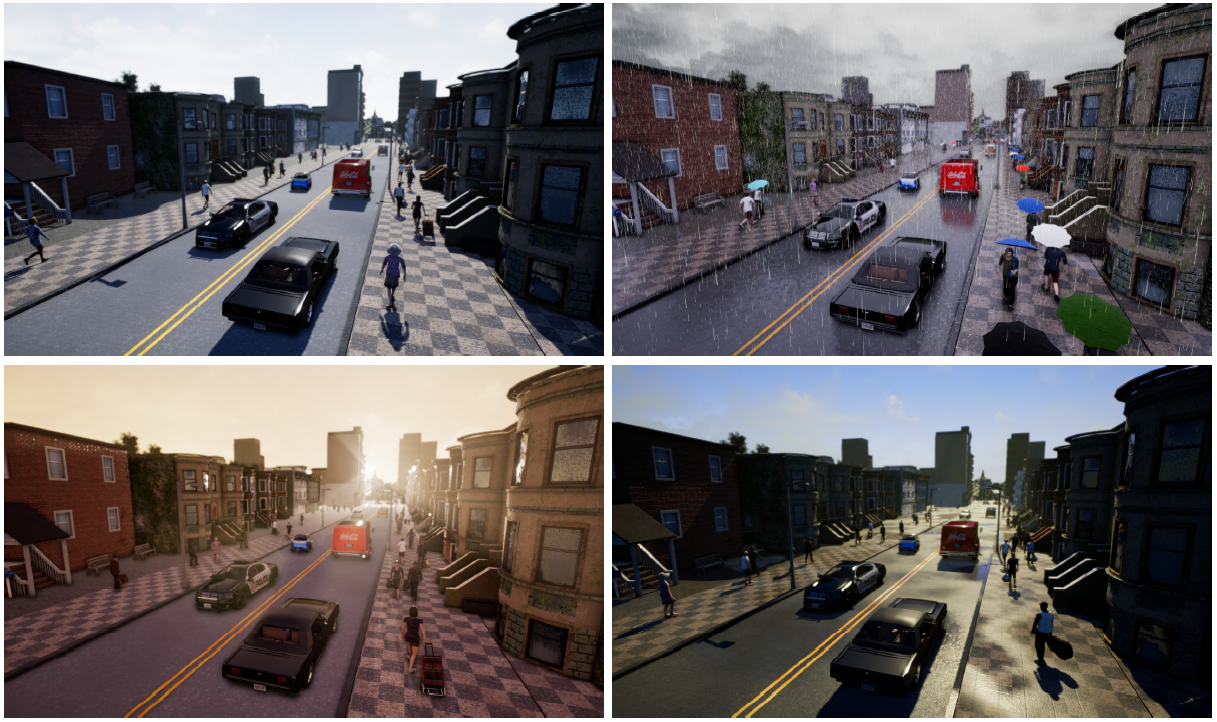
\includegraphics[width=1.0\textwidth]{Images/CARLA_allweather.png}
    \caption[Scenes from the CARLA simulator in different weather conditions]{Scenes from the CARLA simulator in different weather conditions. Clockwise from top left: Day time, Rain, Shortly after rain, Sunset}
    \label{fig:CARLA}
  \end{figure}
\subsection{LGSVL}
LG Silicon Valley Lab (LGSVL) is an open-source simulation engine developed by LG Electronics. It utilizes the Unity gaming engine to render photorealistic environments and taking advantage of technologies like the High-Definition Render Pipeline (HDRP) from Unity. 

This simulator is developed in two parts: the Simulation Engine and the User Autonomous Driving (AD) Stack \cite{lgsvl}. The Simulation Engine, a customizable open-source platform, receiving its inputs from AD stack and simulate the environment, sensors, and vehicle dynamics. The AD Stack comprises three major layers: Perception, Planning, and Control, offering various user-configurable functionalities. The AD Stack and the Simulation Engine is connected through communication bridge interface, such as Cyber RT, ensuring seamless integration \cite{lgsvl}. While the simulator comes with various default sensors including cameras, LiDAR, and Radar, its unique feature lies in its adaptability. Users can build and configure their own sensors and importing models of real-world sensors as plugins. For instance, the plugin for Velodyne VLP-16 LiDAR replicates point cloud generation similar to its actual counterpart. These sensors' data and its mounting positions are defined through JSON-formatted text, simplifying their utilization. Figure \ref{fig:LGVSL} showcases the array of default sensors available within this simulator.

\begin{figure}[h]
    \centering
    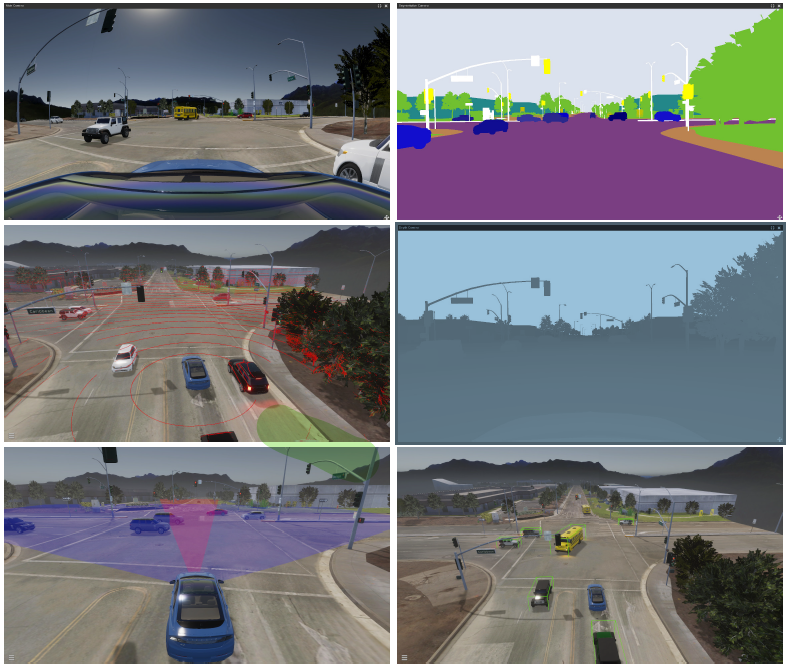
\includegraphics[width=1.0\textwidth]{Images/LGVSL_Sensor.png}
    \caption[Different types of sensors used in LGSVL Simulator]{Different types of sensors. Left (top to bottom): Fish-eye camera, LiDAR, Radar; Right (top to bottom): Segmentation, Depth, 3D Bounding Box.}
    \label{fig:LGVSL}
  \end{figure}

\subsection{SUMMIT}
SUMMIT (The Simulator for Urban Driving in Massive Mixed Traffic) is an open-source simulator developed as an extension of the CARLA simulator \cite{Carla}, inheriting its physics and visual realism. Unlike many other simulators that predominantly which simulate rule-based traffic with minimal randomness, SUMMIT stands out for its ability to replicate the aggressive and chaotic nature of real-world traffic. This distinctive feature attracts users interested in training and testing algorithms for vehicles navigating unregulated traffic scenarios. SUMMIT employs the 'Context-GAMMA', a velocity-space optimization crowd behaviour algorithm \cite{SUMMIT} to simulate traffic behaviour geometrically and topologically. Additionally, it utilizes real-world maps from OpenStreetMap, extracting features such as roads, sidewalks, and roundabouts which are incorporated into the simulator, enabling the replication of real-world maps. An illustrative example can be seen in Figure \ref{fig:summit_both}, which showcases the comparison between a real map and its counterpart with unregulated traffic behaviour in SUMMIT at the Magic Roundabout in England. 

\begin{figure}[h]
  \centering
  \begin{subfigure}{0.49\textwidth}
    \centering
    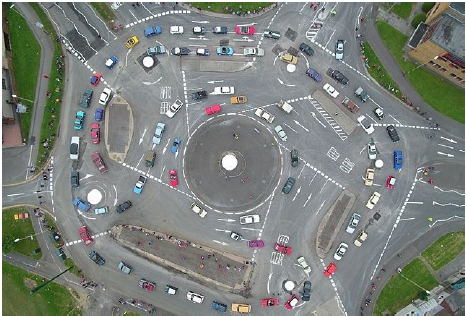
\includegraphics[width=\linewidth]{Images/Summit_org.png}
    \caption{Real map}
    \label{fig:summit_or}
  \end{subfigure}
  \hfill
  \begin{subfigure}{0.49\textwidth}
    \centering
    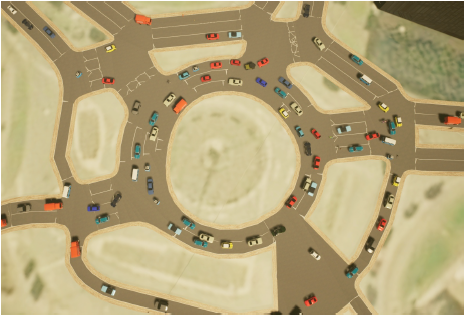
\includegraphics[width=\linewidth]{Images/Summit_sim.png}
    \caption{Simulated map}
    \label{fig:summit_sim}
  \end{subfigure}
  \caption{Scenes in the real world and corresponding scenes in SUMMIT}
  \label{fig:summit_both}
\end{figure}

\subsection{Gazebo}

Gazebo \cite{Gazebobase} stands as a prominent open-source simulator extensively utilized in the field of robotics and autonomous systems. Originating from Carnegie Mellon University in the early 2000s, its primary focus remains on mobile robots. What distinguishes Gazebo from other simulators is its ability to accurately emulate the physics of non-player elements within the environment.
This simulator integrates the Open Dynamics Engine \cite{opende}, crafted by Russel Smith, a widely adopted physics engine within the open-source community. Tailored to replicate the dynamics and kinematics associated with articulated rigid bodies, this engine boasts a comprehensive range of features. These includes various joints, collision detection, mass and rotational functions, as well as a multitude of geometries, including arbitrary triangle meshes.

Gazebo's adaptability is another notable aspect, enabling the concurrent simulation of up to ten robots. This capability proves advantageous particularly in applications involving multiple robots, such as within the domain of autonomous driving. The inclusion of multiple robots, sensors, and actuators, collectively referred to as a model, is seamlessly facilitated through APIs, allowing easy integration into the simulator. Furthermore, Gazebo extends its functionality by facilitating the effortless addition of new 3D user-defined objects using OpenGL, a standard library for 3D object creation. Additionally, GLUT (OpenGL Utility Toolkit) \cite{opengl} offers an interactive user interface, enhancing its accessibility and usability.

While Gazebo excels in accurately simulating various physical phenomena, the challenge arises when attempting to replicate the extensive environments requisite for real-world autonomous driving scenarios. Despite this limitation, owing to its open-source nature, users actively engage in developing custom simulators tailored to their specific requirements such as Gazebo golf cart \cite{golf} which is developed for autonomous golf cart mobility within the golf field.

\subsection{TORCS}
TORCS \cite{torcs}, or The Open Racing Car Simulator, was developed in the early 2000s as an open-source platform for simulating car races. Its standout feature is its ability to adjust car settings, which is crucial in racing simulations. The engine uses a method called discrete-time simulation, where equations are processed in small steps of 0.002 seconds. In TORCS, participants are called "robots" and are loaded as separate parts of the system. This setup allows developers to create new smart agents that follow basic rules for robot code.

TORCS is good at mimicking real racing situations, including how cars move, track designs, weather changes, and interactive settings. This flexibility also makes it useful for academic purposes, letting researchers test artificial intelligence, machine learning, and self-driving algorithms. 

However, there are challenges, like handling complex simulations and making the interactions between cars and the environment more realistic. TORCS benefits from a lively community of developers, researchers, and racing fans because it's open-source, letting people collaborate and improve the platform together.

\section{Comparative Study on Simulators}
This section examines notable studies that compare existing autonomous vehicle simulators and summarizes their approach and results.

In Guan Yang et al. work (2021), "Survey on Autonomous Vehicle Simulation Platforms," \cite{yangsurvey} the team extensively researched different autonomous vehicle simulation platforms. The objective of a simulator is broken down into five parts: Static environment simulation, Dynamic environment and behaviour simulation, Traffic flow simulation, Sensor simulation, and Vehicle dynamics simulation. They also established a taxonomy for existing simulators, categorizing them into Point Cloud-based and 3D Engine-based platforms. Point-based simulators, such as CarCraft from Waymo and Apollo from Baidu, reconstruct the environment based on simulated sensor data. Figure \ref{fig:apollo} displays the map from Apollo, a point-based simulation platform. On other hand, 3D engine-based platforms, like PanoSim, utilize gaming engines like Unity and Unreal to render environments following laws of physics (Figure \ref{fig:Panosim}) \cite{yangsurvey}.
\begin{figure}[H]
  \centering
  \begin{subfigure}{\textwidth}
    \centering
    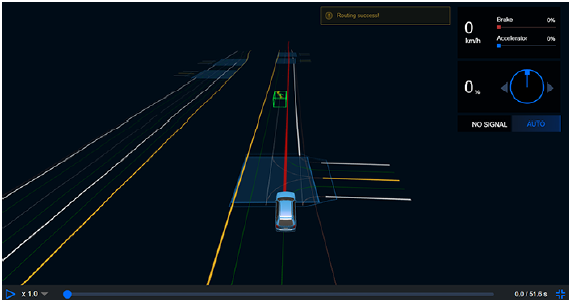
\includegraphics[width=0.75\linewidth]{Images/Apollo_sim.png}
    \caption{Apollo Simulator}
    \label{fig:apollo}
  \end{subfigure}
  
  \vspace{1cm} % Adjust the vertical space between images as needed
  
  \begin{subfigure}{\textwidth}
    \centering
    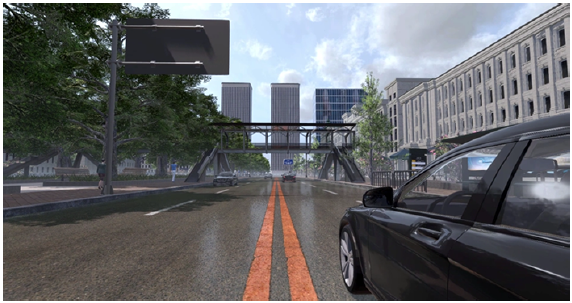
\includegraphics[width=0.75\linewidth]{Images/Panosim.png} 
    \caption{PanoSim Simulator}
    \label{fig:Panosim}
  \end{subfigure}
  
  \caption{Point Based and 3D engine based Simulators}
  \label{fig:taxonomy_based_on_render}
\end{figure}

They further created a table comparing some of popular and relevant simulation platforms and their features as shown in figure \ref{fig:comparison table} \cite{yangsurvey}

\begin{figure}[H]
    \centering
    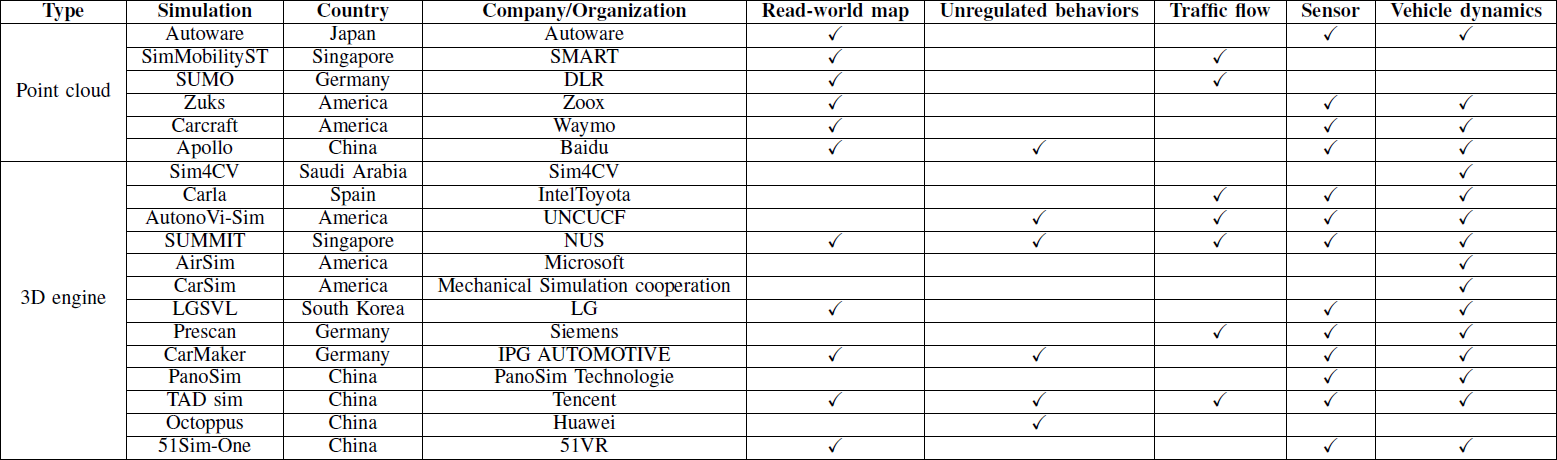
\includegraphics[width=1.0\textwidth]{Images/Comparision Table.png}
    \caption{A Comparison table of various simulator}
    \label{fig:comparison table}
  \end{figure}
Although this table aids in comparing simulators roughly, it doesn’t compare sufficient features for making a concrete decision, and lacks a single metric defining the level of usability of the simulator for a user. While the categorization of simulators is provided, a clear comparative method among simulators is not clearly defined.
In Md Salman Ahmed et al.'s work (2016), an extensive study on connected vehicle simulators was presented \cite{Ahmedsurvey}. The focus was on the domain of connected vehicles, including vehicle-to-vehicle and vehicle-to-server communication. The paper assessed several simulators based on their memory consumption, computing environment (Sequential or Parallel), and the number of vehicles they could handle. However, these results are specific to the connected vehicle domain and may not be applicable to other types of autonomous vehicle simulators effectively.
\section{Generative Adversarial Network}
Generative adversarial networks (GAN) mark a significant advancement in the domain of Generative AI, first introduced in 2014 by Goodfellow et al. in the paper "Generative Adversarial Networks" \cite{7_gan}. Since then, GANs have gained substantial momentum in the field of Generative AI especially in image generation. This section discusses some noteworthy works within the domain of GANs.
\subsection{VGAN(Video Generative Adversarial Network)}
VGAN, developed by Carl Vondrick et al. \cite{8_Vgan}, specializes in generating videos with its scene dynamics. The model is capable of generating videos up to a second at full frame rate. Its training involves over 2 million pre-processed videos sourced from the internet, categorized into four distinct groups: golf courses, hospital rooms, beaches, and train stations.

The architecture of VGAN employs a standard Generator-Discriminator structure. The generated video is segmented into two features: foreground and background, assuming a fixed camera resulting in a static background. The generator comprises two network streams dedicated to foreground and background, respectively. The foreground stream consists five layers of 3D spatiotemporal convolution layers (time x width x height), which upsamples the information from a low-dimensional latent code $z$, sampled from a standard normal distribution. A masking layer $m$ is introduced before the final layer, outlining the pixels of objects in the foreground. Meanwhile, the background stream utilizes five layers of 2D convolution layers (width x height), responsible for generating a background $b$. The background stream uses 2D convolution layers as the background is assumed to be same for all the generated frames. The synthesis of foreground and background follows the equation: $m \cdot f + (1 - m) \cdot b$


The resultant video, comprising 32 frames with dimensions of 64x64, is generated from a 100-dimensional latent code sampled from a normal distribution. The Discriminator is designed for two primary objectives: classifying realistic scenes and recognizing plausible and smooth motion between frames. It mirrors the architecture of the foreground stream of generator with a five-layered spatiotemporal convolutional setup, employing downsampling instead of upsampling. The final layer outputs a binary classification (real or not). Batch normalization and ReLU activation functions are used after every layer in both the generator and discriminator. The VGAN is trained using Adam optimizer with a batch size of 64. Results demonstrate the model's ability to generate videos with a sharp background and a slightly blurry foreground. While the resolution of the foreground might be blurred, the motion of the generated foreground is convincing. However, the user had no control over the content of generation. Figure \ref{fig:vgan} illustrated the frames of various generated videos.

\begin{figure}[H]
    \centering
    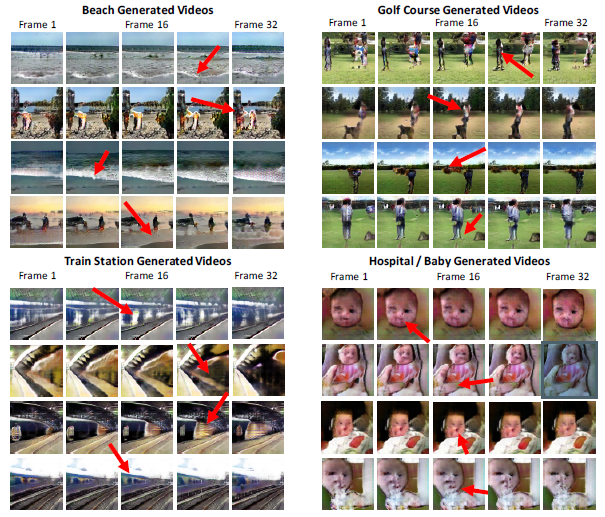
\includegraphics[width=0.75\textwidth]{Images/vgan.png}
    \caption{Frames of Videos generated by VGAN}
    \label{fig:vgan}
  \end{figure}

\subsection{RV GAN}
The RV-GAN, introduced by Sonam Gupta et al., \cite{rvgan}stands for Recurrent Variational Generative Adversarial Network and serves the purpose of unconditional video generation. This particular GAN employs a specialized variant of LSTM known as TransConv LSTM. The innovation lies in modifying the conventional ConvLSTM by integrating a transpose convolutional structure into its input-to-state transitions. This unique design allows the network to simultaneously capture spatial and temporal relationships across layers within the TC-LSTM unit. (See Figure \ref{fig:transconv} for a diagrammatic representation of the TransConv LSTM \cite{rvgan}.)

\begin{figure}[H]
    \centering
    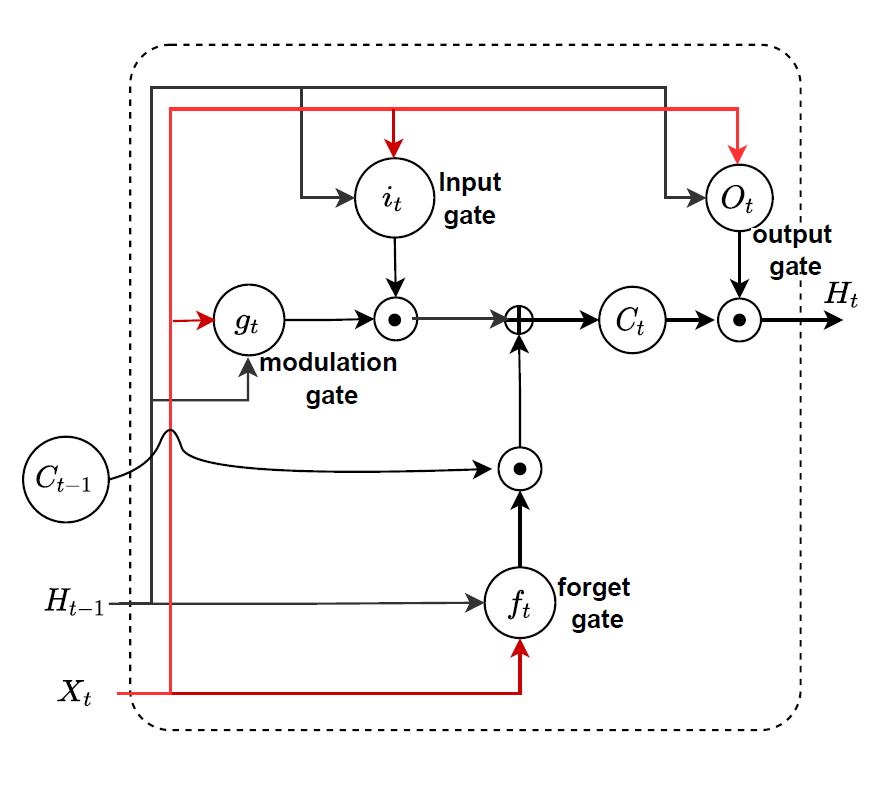
\includegraphics[width=0.70\textwidth]{Images/transconv.png}
    \caption[ Diagrammatic representation of the TransConv LSTM]{Diagrammatic representation of the TransConv LSTM. Ht−1,Ct−1,Ht,Ct are the hidden states and cell states at previous and current timestamps. Xt is input to the TC-LSTM unit.\cite{rvgan}}
    \label{fig:transconv}
  \end{figure}

Figure: Diagrammatic representation of the TransConv LSTM. Ht−1,Ct−1,Ht,Ct are the hidden states and cell states at previous and current timestamps. Xt is input to the TC-LSTM unit.
The composite model comprises a generator built with blocks of TC-LSTM units and incorporates 2 discriminators similar to Mcocgan \cite{10_mocogan}. In the generator, noise sampled from a random distribution is fed at each time step, along with the inputs of the hidden state and cell state from the preceding time step to account for temporal information. This process generates frames that exhibit strong correlation with previous ones. On the other hand, the discriminator is structured using 2D and 3D convolution layers, specifically for image and video discrimination, respectively. The entire network is trained on the combined loss function derived from both discriminators.
Training of the model occurs on datasets such as Weizmann \cite{weizmann}, UCF101\cite{UCF}, and MUG\cite{13_MUG}, with evaluation based on the Frechet Inception Distance metric (FID) \cite{fid}. Due to its recurrent structure, the proposed method demonstrates the ability to generate high-quality videos, extending up to 2 times the length (32 frames) of the training videos during inference. The authors substantiate the versatility of this GAN by showcasing its adaptability to class conditional video generation. RV-GAN exhibits superior performance compared to most other methods, falling short only when compared to V3GAN\cite{v3gan} on UCF101.

\subsection{Imaginator}
ImaGINator is a conditional Generative Adversarial Network (GAN) developed by Yaohui Wang et al \cite{9_imaginator}. Its primary aim is to produce human videos depicting various expressions. Unlike VGAN \cite{8_Vgan}, this model generates videos conditioned on specific class labels for expressions for example smiling, jogging... The model is designed to segment the generated video into spatial and temporal parts.

ImaGINator comprises a generator and two discriminators. The generator adopts an encoder-decoder architecture with skip connections. It takes a static image featuring a person's face as input and encodes it into a latent vector $p$.  In addition, this vector is concatenated with one-hot encoded class label $c$, representing the expression, and random noise sampled from a standard normal distribution. This fusion embeds spatial ($p$) and temporal information ($c$) into the latent vector. The decoder, structured as a (1+2)D convolution layer, explicitly separates temporal and spatial information. It mirrors the dimensions of the encoder's architecture and had skip connections from encoder, ensuring that each decoder layer retains embedded spatial details from the corresponding encoder layer. Moreover, the embedded class label vector is integrated into every decoder layer, ensuring the preservation of temporal information throughout the model. The generated video consists of a fixed number of frames and the last layer of the generator outputs an image with all the frames.  

Two discriminators serve distinct purposes: '$d_i$' evaluates individual frames of the generated video to classify real from fake based on appearance, while '$d_v$' examines the sequence of frames alongside the class label to classify the dynamics within the frames as real or fake. The Generator is optimized on the combined loss function from both discriminators and a reconstruction loss for corresponding frames. Each discriminator's loss function optimizes the weights of corresponding discriminator. The ADAM optimizer with the same learning rate is used across all generator and discriminator components.
\begin{figure}[H]
    \centering
    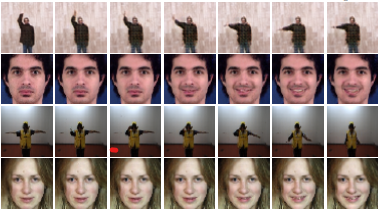
\includegraphics[width=0.6\textwidth]{Images/Imaginator.png}
    \caption{Frames of  video generated by Imaginator}
    \label{fig:Imaginator}
  \end{figure}
  
Evaluation metrics such as Frechet Inception Distance (FID), Peak Signal-to-Noise Ratio (PSNR), and Structural Similarity Index Measure are used to evaluate the performance of the generated videos and to monitor the training progress. Figure \ref{fig:Imaginator}  provides a visual representation of the frames within the generated video. 

The model was trained on various widely used datasets like MUG Facial Expression Dataset \cite{13_MUG}, NATOPS Aircraft Handling Signal Dataset \cite{14_aircraft}, Weizmann Action Dataset \cite{15_act_rec}, and UvA-NEMO Smile Dataset \cite{16_face}. Comparative analysis shows the superior image quality compared to VGAN. Furthermore, the model's ability to control the content of generated videos using class labels holds significant potential across various applications.
\subsection{MoCoGAN}
Motion and content decomposed GAN (MoCOGAN), a Video Generation GAN introduced by Sergey Tulyakov et al. in 2016 \cite{10_mocogan}, operates on a unique architecture that segments videos into Content and Motion. This segmentation allows the model to sample inputs separately from the Content and Motion subspaces (unsupervised). Notably, this architecture enables the model to generate videos depicting the same content with different actions or the same action with different content. While designed for shorter video durations, MoCOGAN doesn't require a fixed length for the generated videos. Given the shorter duration, the video's subject is assumed to remain constant.

The model comprises four networks: a Recurrent Neural Network ($R_m$), Generator ($G_1$), Image Discriminator ($D_i$), and Video Discriminator ($D_v$). The Generator sequentially produces frames by taking a latent image $Z$ as input, containing $z_c$ and $z_m$. The random vector $z_c$ represents the video's content and is sampled from a content subspace, remaining constant throughout the video as the subject remains unchanged. On the other hand, the latent vector "$z_m$", which determines the motion trajectory of the subject, and it is recursively outputted by Rm by sampling from a motion subspace at each timestep.

The $R_m$ parameters are learned during training, as not all motion trajectories are physically possible. The generator $G$ takes $Z$ (combination of $z_c$ and $z_m$) and generates video frames sequentially. The Image Discriminator assesses frame quality, while the Video Discriminator evaluates subject motion in the video. The RNN is trained exclusively on the Video Discriminator loss, while the entire Generator network is trained on the combined loss of the discriminators.

The model's training utilizes the Weizmann Dataset \cite{15_act_rec} \ref{fig:moco1} and Tai-Chi Dataset \cite{17_taichi} \ref{fig:Moco2}, and its performance was assessed using the Average Content Distance (ACD). Visual representations in Figure \ref{fig:moco} depict video clip frames generated by the MoCoGAN model.
\begin{figure}[htb]
    \centering
    \begin{subfigure}{0.6\textwidth}
        \centering
        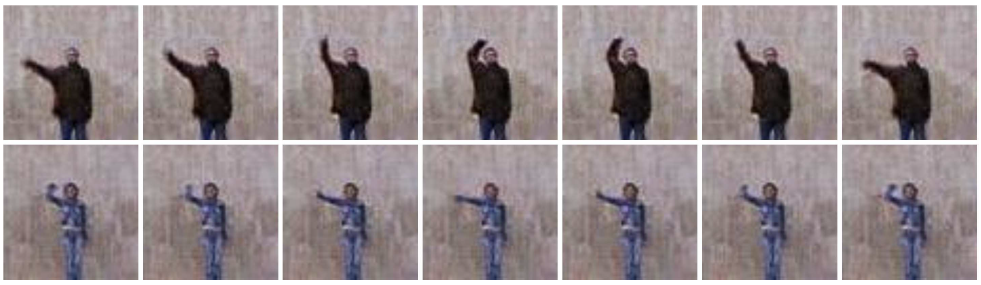
\includegraphics[width=\linewidth]{Images/Moco1.png}
        \caption{Weizmann Dataset}
        \label{fig:moco1}
    \end{subfigure}
    \hfill
    \begin{subfigure}{0.6\textwidth}
        \centering
        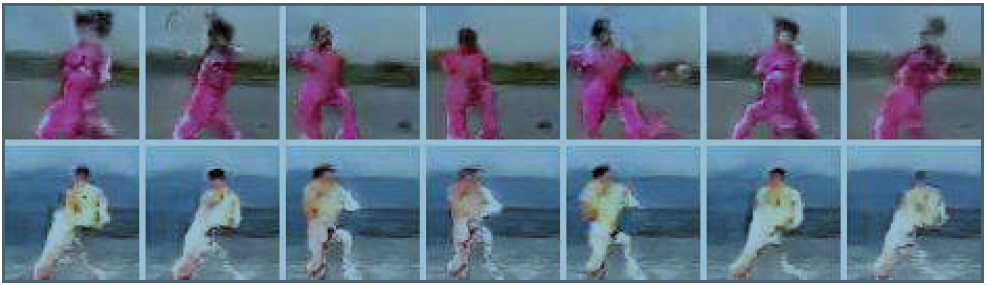
\includegraphics[width=\linewidth]{Images/Moco2.png}
        \caption{Tai-Chi Dataset}
        \label{fig:Moco2}
    \end{subfigure}
    \caption{Frames of video generated by MoCoGAN}
    \label{fig:moco}
\end{figure}
Notably, MoCoGAN had outperformed VGAN \cite{8_Vgan}and TGAN \cite{tgan} in image quality within the videos and offers the flexibility of generating videos of varying lengths. However, it lacks direct control over content creation like Imaginator as content is randomly sampled from the content subspace
\subsection{Pix2Pix GAN}
Pix2Pix, introduced in 2016 by Philip Isola et al \cite{11_image2_image}, is an image translation technique using Conditional GANs. Image translation involves transforming images from one domain to another, such as converting grayscale images to colour images. In \cite{12_pix2pix}, the method was applied to translate satellite terrain images into Google Maps style images. 

The structure of the conditional GAN resembles that of a Normal GAN, comprising a Generator and a Discriminator. In \cite{12_pix2pix}, the generator adopts an encoder-decoder architecture, where the encoder consisting of blocks that include a convolution layer, Batch Normalization, and ReLU activation function. The decoder mirrors the encoder, employing skip connections (known as U-Nets) between corresponding layers to retain information and prevent loss during transmission through bottle necks \cite{11_image2_image}. The Generator takes an image from the input domain and produces an image in the target domain. On the other hand, the Discriminator intakes the paired images from both domains, uses standard convolutional layers, converging in a final layer that determines the given image (real or fake). Using PatchGAN, the Discriminator segments images into 70x70 patches and performs binary classification for each patch, this makes the discriminator suitable for any given image size.

Training involves computing the reconstruction loss between the generated image and the target image. The generator's gradients are optimized to minimize this loss. The composed model training combines the Discriminator loss and the reconstruction loss using a weighted sum for gradient update. The dataset used for training, consisting of 1097 paired images of satellite and Google Maps images. Each image is pre-processed and rescaled to 256X256 pixels before training. Figure \ref{fig:p2p} illustrates the satellite images and its corresponding google map image and generated image.
\begin{figure}[htb]
    \centering
    \begin{subfigure}{0.6\textwidth}
        \centering
        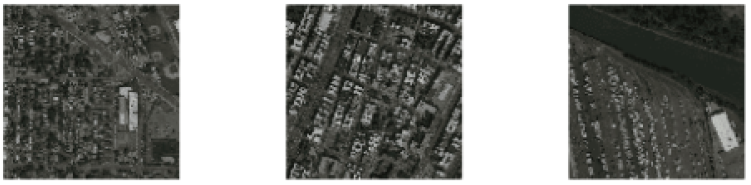
\includegraphics[width=\linewidth]{Images/pix2pix1.png}
    \end{subfigure}
    \hfill
    \begin{subfigure}{0.6\textwidth}
        \centering
        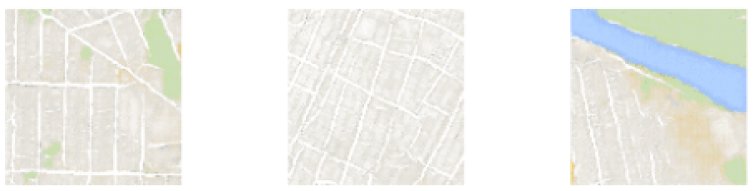
\includegraphics[width=\linewidth]{Images/pix2pix2.png}
    \end{subfigure}
    \hfill
    \begin{subfigure}{0.6\textwidth}
        \centering
        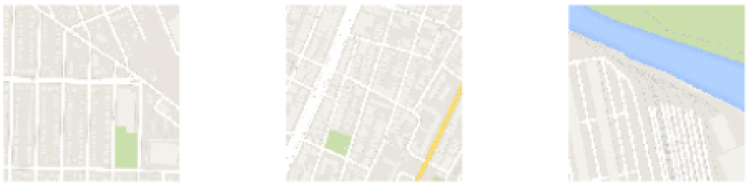
\includegraphics[width=\linewidth]{Images/pix2pix3.png}
    \end{subfigure}
    \caption[Frames of video generated by Pix2Pix GAN]{The satellite images [top] and its corresponding google map image [middle] and generated image after 10 epochs [Bottom]}
    \label{fig:p2p}
\end{figure}

While image translation using this method has diverse applications, this method often requires paired datasets, which is difficult to obtain in most of the cases.
\chapter{Framework for Comparative Study}
The suitability of an autonomous vehicle simulator for a particular user varies significantly based on several factors. These factors include various aspects such as the intended application, sensor support availability, integration of real-world components like vehicles and maps, computational resources... Within this proposed method 73 such parameters are identified and these parameters collectively contribute to formulate a single score for each simulator. This score serves as a means for comparison between different simulators. 
\section{Comparison Parameters}
The identified parameters are categorized into six broad classifications: Sensors, Actors, Environment, Vehicle, Framework, and Algorithm. Each parameter is evaluated using a scoring system ranging from 0 to 1 where 0 being worse and 1 is best. In cases of binary classification, where a feature's availability is assessed, the corresponding parameter receives a score of 0 if the feature is unavailable and 1 if it is available.
\subsection{Sensors}
Sensors serve as the tool to perceive the vehicle's surrounding environment. They play a crucial role in driverless vehicles by providing inputs to the algorithm, which determines subsequent actions of the vehicle. In autonomous vehicles, multiple sensors are commonly utilized simultaneously. It is important to accurately model and integrate these sensors within the simulator to mimic those employed in real vehicles. This part examines the various aspects of sensors that can be used within an autonomous vehicle simulator.
\subsubsection{Default Sensors}
The majority of simulators offer some default sensor models that are readily available for use. A simulator will receive a score of 1 for each sensors defined below if it offers support for it; otherwise, it will be assigned a score of 0.
\begin{enumerate}[label=\alph*.]
    \item RGB Camera \\
    An RGB camera functions by translating the 3D environment within its field of view into a 3-channel 2D image (Red, Green, Blue). Refer to Figure \ref{fig:RGB} \cite{senimage} for an example of data captured by an RGB camera mounted on a vehicle. These images are valuable for understanding the surroundings, including aspects such as traffic lights, signage, and pedestrian crossings.

    
    \begin{minipage}[t]{\linewidth}
        \centering
        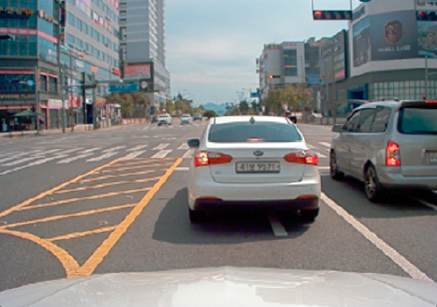
\includegraphics[width=0.75\textwidth]{Images/RGB.png}
        \captionof{figure}{Image of vehicles surroundings captured by a RGB camera}
        \label{fig:RGB}
        \vspace{-\baselineskip} % Adjust spacing if needed
    \end{minipage}
    \hfill
    
    \item Depth Camera \\
    A depth camera captures a single-channel image embedding depth information. Each pixel in this image denotes the distance between the camera's mounting point and objects in the 3D environment it references. Figure \ref{fig:depth} showcases an example data captured by a Depth Camera fixed on a vehicle. This data is commonly utilized to measure distances between the ego vehicle and other nearby vehicles.
    \begin{minipage}[t]{\linewidth}
        \centering
        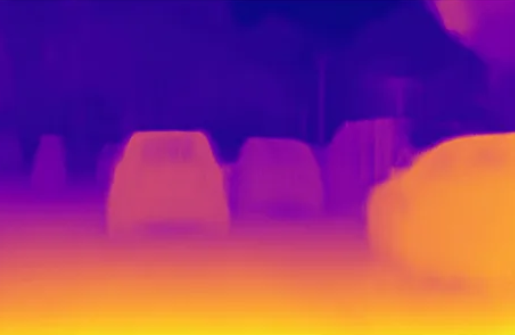
\includegraphics[width=0.75\textwidth]{Images/Dethcam.png}
        \captionof{figure}{Depth Image of vehicles surroundings captured by a depth camera}
        \label{fig:depth}
        \vspace{-\baselineskip} % Adjust spacing if needed
    \end{minipage}
    \hfill
    
    \item 3D Lidar \\
    Unlike traditional cameras, the 3D lidar creates a 3D point cloud representation of the environment. Each voxel's position corresponds to a point on objects in the surroundings. This sensor projects laser beams and calculates positions based on time of flight. Figure \ref{fig:pointcloud} \cite{senimage} illustrates an isometric view of a point cloud generated by 3D lidar. However, factors such as fog or object texture can distort the energy of the laser signals. These sensors are occasionally affixed to a rotary motor to achieve a 360-degree scan around the device.
    \begin{minipage}[t]{\linewidth}
        \centering
        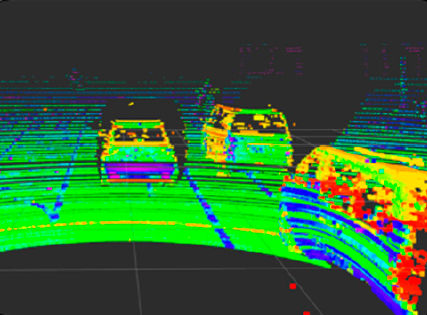
\includegraphics[width=0.75\textwidth]{Images/Lidardata.png}
        \captionof{figure}{Point cloud projection of surrounding captured by 3D Lidar}
        \label{fig:pointcloud}
        \vspace{-\baselineskip} % Adjust spacing if needed
    \end{minipage}
    \hfill
    
    \item Radar \\
    Similar to the 3D lidar, the Radar sensor maps the environment into a 3D point cloud. However, unlike the 3D lidar, this sensor uses electromagnetic (EM) waves instead of laser beams. Radars takes the advantages of EM waves such as covering longer distances and experiencing less distortion from external factors. Both the 3D lidar and Radar are utilized to project the surrounding environment in 3D data.
    
    \item IMU Sensor \\
    The Inertial Measurement Unit (IMU) sensor measures specific forces like acceleration and angular velocity. It provides information about the orientation and changes in position of the vehicle on which it is mounted on. IMU consists of sensing elements such as accelerometers and gyroscopes which aids in determining the vehicle's acceleration, change in direction, and rotation.

    \item Semantic Information \\
    Semantic Information isn't a physical sensor used directly in autonomous vehicles. Rather, it denotes a simulator's ability to offer semantic information about every object within the environment. This information typically includes the class or name of objects, such as trees, dogs, children, women, along with the coordinates of bounding boxes encapsulating these objects. Refer to Figure \ref{fig:sem} \cite{senimage} for an illustration of the environment with bounding boxes and class labels of the objects. This information can be valuable in certain training algorithms like reinforcement learning, facilitating the provision of rewards and penalties.
    \begin{minipage}[t]{\linewidth}
        \centering
        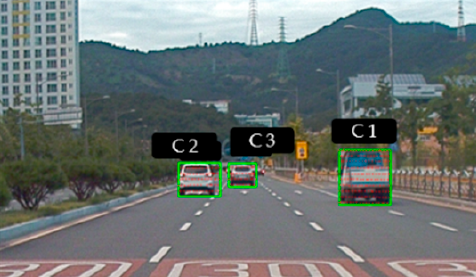
\includegraphics[width=0.75\textwidth]{Images/semantic.png}
        \captionof{figure}{Semantic Information of cars in environment with bounding boxes}
        \label{fig:sem}
        \vspace{-\baselineskip} % Adjust spacing if needed
    \end{minipage}
    \hfill
    \item Force Impact sensor \\
    This sensor measures the force experienced by a vehicle during impact with another object. This measurement directly correlates with the damage caused by both the vehicle and the object. Moreover, it can be utilized to assign weighted rewards and penalties.

    \item Fuel/Battery Sensor \\
    This sensor monitors information regarding fuel or power consumption by the vehicle. As self-driving vehicles aim for efficiency, researchers worldwide continually work to enhance fuel efficiency of the vehicle. Therefore, it's crucial for a simulator to offer such data.

    \item Vehicle Speed Sensor\\
    A widely used sensor present in nearly all vehicles, it measures the vehicle's velocity. This sensor is particularly important when navigating in areas with speed limits, such as city roads or warehouses within the simulator.

    \item GPS \\
    The Global Positioning System (GPS) is a geolocation sensor utilized for locating and navigation. It's one of the most common sensors found in commercial vehicles, essential for path planning both on roads and within closed environments. Regarding simulators, it's vital for them to provide information about the coordinates of the vehicle and its destination within global boundaries with respect to the simulator scale.

    \item Visibility Sensor\\
    Visibility while driving can be affected by various environmental factors like fog, smog, or pollution. It is a measure of the maximum distance at which objects can be clearly seen which plays a critical role in safe driving. For simulators, providing this information becomes crucial, particularly when simulating foggy conditions. 

    \item Other Vehicle Sensors related to Vehicle Dynamics \\
    Conventional cars possess numerous sensors measuring various car properties such as tire pressure, parking aid, engine RPM. However, not all these vehicle sensors are typically utilized in autonomous vehicle research. An ideal simulator should offer the infrastructure to model any of these vehicle sensors when needed, quantifying its ability to define and provide data related to ego vehicle.
    
    \item Other Environment Sensors related to Perception \\
    This parameter denotes the user's ability to define sensors measuring environmental properties. These user-defined sensors could offer data regarding the car's surroundings, like the number of people/vehicles within the car's field of perception. For example, sensors like audio recognition for identifying priority vehicles, such as ambulance and fire-fighting vehicles, fall under this category.
    
    \item Macroscopic Global Sensors \\
    Another user-defined sensor, this provides information about the simulation world, not just the local area near the vehicle. Such a sensor could furnish global details like traffic conditions in specific sections of the map or future weather forecasts, which can significantly aid in path planning.    
\end{enumerate}

\subsubsection{Multiple Synchronous Sensors}
In autonomous vehicles, multiple sensors are commonly used simultaneously to enhance reliability and provide backup in case of sensor failure. Simultaneous data from multiple sensors provide more dependable information compared to a single sensor. An AV simulator's capability to handle multiple synchronized sensor models and provide their data becomes crucial. This parameter ensures the synchronized data simulated by multiple sensors at a given time corresponds to the same time step and is coherent with each other.

\subsubsection{User-Defined Sensor Position and Orientation}
The placement and orientation of sensors within a vehicle significantly influence their application. AV Engineers meticulously design the mounting points and orientations, especially when multiple sensors are used to avoid sensor blind spots. This parameter evaluates a simulator's capacity of enabling users to define sensor location and orientation with respect to the vehicle geometry.

\subsubsection{Precision of Sensor Readings}
Sensor precision refers to the smallest measurable change in a sensor's readings. This attribute applies to various sensor types and their measurements. The precision of a sensor varies based on application needs and accuracy required. An adaptable simulator should accommodate diverse levels of precision, allowing users to configure it for various sensor according to their requirements.

\subsubsection{Real-Time Sensor Models}
Some vehicle manufacturers develop unique in-house sensors with unique features. Simulators incorporating digital models of these sensors help users to retain their specific functionalities within the simulation. Additionally, providing digital models of popular sensors readily available in the market becomes advantageous. This parameter evaluates a simulator's capability to import real-time digital models of sensors and integrate them into the simulation environment.

\subsubsection{User-Defined Sensors and Observers}
In the dynamic field of autonomous driving, new sensor technologies are frequently emerging, and existing sensors undergo performance updates to better understand the environment. Within a simulator, users might have specific data of interest for their application or need to monitor certain aspects. The simulator's capability to enable users to define observers to monitor data or model new sensors becomes important to cope up with evolving sensor needs and user-specific requirements.

\subsection{Actors}
Actors within the simulator constitute the diverse objects forming the environment. These actors broadly categorize into stationary and non-stationary, with stationary actors maintaining fixed positions (e.g., buildings, trees, traffic signs) and non-stationary actors changing their positions during simulation (e.g., people, animals, moving vehicles). This part explores criteria of various parameter related to actors that influences the comparison. 
\subsubsection{Geometry}

\begin{enumerate}[label=\alph*.]
    \item Predefined Scenarios\\
    Environments for vehicle operation vary widely such as rural, urban, industrial… each possessing unique features and actors. For instance, observing a child is less likely in an industrial setting compared to seeing a cargo truck. This parameter evaluates a simulator's capability to offer presets of environments with appropriate actors corresponding to various scenarios.
    
    \item Predefined Models for Actors\\
    This parameter evaluates the simulator's ability to offer access to meticulously designed digital assets (actors) across various categories such as buildings, vehicles, people, and traffic signs. These models are pre-configured across various scenarios and ready for deployment within the simulator environment.
    
    \item User-Defined Actors\\
    Apart from the preconfigured libraries of 3D models, the simulator should allow users to import custom 3D models of actors while maintaining a standardized scale within the simulator. This feature can aid user to tailor the simulator for their use case. For example, develop a simulator for driverless vehicle in golf field demands integration of 3D models of golf carts and players.
    
    \item Number of Actors and Spawning Location\\
    The nature of an environment is influenced by the number of actors within it. Users should have the ability to adjust the number of actors and their location to configure the environment. For example, configuring the traffic density in a particular road by defining number and location of vehicles or placing specific objects like traffic light poles.
    
    \item Recreation of Real-Time Models\\
    Simulators should possess real-time 3D models of actors such as cars, buildings while preserving their physical properties like geometry and textures. This feature appeals to users working with real-time vehicles or entities.
    
    \item Path/Destination of Actors\\
    Configurability of the moving trajectories for non-stationary actors, allows users to define paths and destinations. Actors should also respawn in new locations when they move beyond environment boundaries. This parameter ensures this capability of a simulator providing flexibility in defining their movement patterns.
    
    \item Context-Aware Spawning \\
    Ensuring that the spawning or respawning of actors aligns with contextual reasoning. For instance, spawning more ambulances near hospitals demonstrates intelligent spawning based on context. This parameter evaluates the simulator's ability to spawn actors sensibly in relation to their surroundings.
    
\end{enumerate}
\subsubsection{Behaviour}
\begin{enumerate}[label=\alph*.]
    \item Predefined Rules\\
    Simulators can define certain preset rules governing actor behaviour, such as traffic regulations in specific countries, readily available for use within the simulation.
    
    \item User-Defined Rules\\
    Allowing users to define specific behaviour patterns for actors within the simulator in addition to predefined rules, provides better customization options.
    
    \item Distinguishable Behavioural Patterns\\
    Simulators aiming to replicate real environments must simulate distinct behavioural patterns among actors. For example, distinguishing between the behaviour of an adult, a child, and a dog walking on a sidewalk. A simulator earns a score of 1 for this parameter if it is capable of accurately simulating these behavioural differences.
    
    \item Sensitivity\\
    Sensitivity refers to an actor's responsiveness or reaction to actions taken by other actors, including the ego vehicle within the environment. A score of 0.5 is given if actors respond solely to the ego vehicle, while a score of 1 is granted if actors respond to all fellow actors. This parameter evaluates the simulator's sensitivity to fellow actors' actions.

    \item Level of Aggressiveness in Driving\\
    The driving pattern varies among various parts of the world. Simulators should allow users to define driving patterns' aggressiveness using metrics like violations per kilometer driven or similar parameters. This parameter enables users to train and test in various driving conditions by defining custom behavioural patterns.
    
    \item Reproducibility\\
    Certain random behaviours exhibited by actors can elicit unique responses from the ego vehicle. The simulator should enable users to reproduce the same set of random actions performed by actors, known as seeding. This parameter evaluates the simulator's capability to reproduce a specific set of actions performed by actors for further analysis.
    
\end{enumerate}

\subsection{Environment}
The simulator's environment includes the weather, terrains, maps, and conditions where the vehicle operates. This part explores various the criteria for various comparative parameters related to environment. 
\subsubsection{Pre-defined Libraries}
This parameter assesses the simulator's capability to feature pre-designed environments consisting of diverse landscape and weather conditions. The simulator earns a score of 0.5 if it satisfies one condition and a score of 1 if it fulfils both.
\subsubsection{User-Defined Environment}
Simulator tools enabling users to define their own maps and various weather conditions enhance customization and adaptability, allowing for efficient simulation tailored to specific needs.
\subsubsection{Real World Maps}
The capability to import or utilize real-world maps within the simulator holds significant importance, particularly for developing commercial autonomous vehicles that directly navigate on real road. A simulator scores 1 if it facilitates user access to import or integrate real-world maps and associated features.
\subsubsection{Photorealism}
Photorealism is the concept of how closely a simulator's environment resembles the real world in appearance. Assessing photorealism is subjective, thus scored by users through visual inspection on a scale of 0 to 1. A simulator that closely replicates reality receives a higher score, while deviations affect the score inversely.
\subsubsection{Variable Resolution}
The ability to vary the level of detail in the rendered environment by adjusting resolution. Variable resolution provides flexibility, allowing users to balance computational resources against information accuracy. With lower resolution considerable computation resources can be saved but potentially losing detail and vice versa. This parameter checks the ability of a simulator which enables the user to vary the resolution.
\subsubsection{Context-Aware Map Planning}
The simulator-generated map should possess contextual coherence, ensuring that elements such as buildings, roads, and traffic lights correlate logically within the environment. This feature scores 1 when a simulator has the capability of generating contextually plausible maps.
\subsubsection{User-Defined Scenarios}
The simulator-generated map should possess contextual coherence, ensuring that elements such as buildings, roads, and traffic lights correlate logically within the environment. This feature scores 1 when a simulator has the capability of generating contextually plausible maps.
\subsubsection{Material Definition}
The optical properties of environment materials can influence sensor data, impacting sensors like Lidar and Cameras. For instance, Lidar may fail to detect glass walls due to the laser beam passing through it rather than reflecting. This parameter evaluates the simulator's capability to enable users to define materials and texture of objects in the environment.
\subsubsection{Variable Level of Sun Shades}
Shades of the sun can influence significantly in replicating the time of day and weather ultimately impacting the sensor readings. This parameter refers to the simulator's ability to allow users to manipulate sun shades, considering factors like time of day and weather.
\subsubsection{Special Optical Features}
Real-world optical phenomena like sun glare, mirage, dust, and fog can impact driver visibility and sensor data for driverless vehicles. Therefore, it's also important for simulators to model these features which impacts sensor data and subsequent vehicle actions.
\subsubsection{Data Visualization and Analytical Tools}
Simulator tools facilitating the display of various data and analyses during training and testing offer valuable insights to users. This parameter assesses whether the simulator allows users to define data visualization and monitoring tools, which could include sensory data from the vehicle, algorithm-related data, or annotations like bounding boxes and semantic truth.
\subsubsection{Rendering}
During testing, the quality of scene rendering aids in analysing algorithm performance. Users should have the ability to modify rendering parameters such as view angle and frames per second, ensuring adaptable display quality. This parameter evaluates the simulator's capability to offer configurable rendering options, earning a score of 1 if available.
\subsubsection{Recording}
Recording the training process allows users to analyse performance and playback sessions for future evaluation. This parameter accounts for the simulator's ability to record the training process alongside associated data, aiding users in comprehensive analysis.

\subsection{Ego Vehicle}
The agent vehicle, or ego vehicle, is the vehicle which is subjected to training or testing for autonomous driving within the simulator. This part explores various parameters evaluating the simulator based on the ego vehicle.

\subsubsection{Vehicle Geometry}
Vehicle Geometry refers to the dimensions and bounding box encapsulating the vehicle in the 3D environment. This parameter evaluates the simulator's capability to allow users to configure the geometry of the ego vehicle.

\subsubsection{Wheel Geometry}
This parameter involves the ability to modify suspension and steering system parameters of the ego vehicle within the simulator. Ensuring adherence to physics related to wheel geometry is important as it impacts driving performance significantly.

\subsubsection{Real-World Models}
This parameter assesses the simulator's feature of enabling the user to import and use of 3D models of real-world vehicles developed by vehicle manufacturers. This feature is important and time saving for researchers from vehicle manufacturing companies.

\subsubsection{Real-World Physics}
This parameter is a check for the simulator's capacity to simulate various physical parameters associated with driving, including wheel slip, crash damage, and vehicle inertial behaviour. Accurate replication of these features is vital for developing algorithms for real-world on-road autonomous vehicles.

\subsubsection{Input Commands}
The driving algorithm generates action commands for the vehicle (e.g., acceleration, steering angle) based on observations. Configurability of input commands for every component within the ego vehicle is crucial to accommodate various algorithms. This parameter ensures the simulator's ability to configure input commands for the vehicle.

\subsubsection{Other Components}
Minor components like headlights and horns can have minor impact in driving. The simulator should allow users to model the intensity or impact of these components. This parameter evaluates the simulator's feature for adjusting the effects of such components.

\subsection{Framework}
The framework within which the simulator operates plays a crucial role in its versatility and usability. This part evaluates various comparative parameter related to simulator’s framework.

\subsubsection{Cross-Platform Compatibility}
This parameter assesses the compatibility of the simulator software across diverse operating systems, determining support for OS environments such as Linux, ROS, Windows, MacOS, and any other relevant OS. The simulator earns a score of 1 for each supported operating system from the listed ones.

\subsubsection{Open Source}
Evaluating whether the simulator or parts of it are open source, enabling users to tailor the simulator to their specific needs by importing components as plugins and developing customized software. A score of 1 is given if the simulator allows for such user-driven customizations.

\subsubsection{Scripting Language Support}
This parameter evaluates the breadth of scripting language support within the simulator, crucial for facilitating communication between users and the simulator. The assessment includes popular languages like Python, C++, C, R, Java, and other relevant scripting languages. The simulator earns a score of 1 for each supported scripting language from the listed options.

\subsubsection{Scalability}
This parameter evaluates the simulator's ability to provide various light versions to suit diverse user needs. Offering various individual light versions with unique features, alongside a comprehensive pro version encompassing all features, the simulator ensures adaptability to different user requirements. This feature contributes to making the software more streamlined and efficient for users by allowing them to opt for lighter versions catering to their specific needs.

\subsubsection{Computational Resource Evaluation}
In this study, the computational resource consumed by a software is calculated based on electrical energy consumption by a baseline system under maximum operation. The configuration of the baseline system and its power consumption at it maximum usage is tabulated in Table \ref{tab:systab}

\begin{table}[htbp]
  \centering
  
  \begin{minipage}{\linewidth}
    \renewcommand{\arraystretch}{1.0} 
    \begin{tabular}{|c|c|c|}
      \hline
      \textbf{Level} & \textbf{Name} & \textbf{Description} \\
      \hline
        Processor & Intel i9 processor & 200--250 Watts \\ \hline 
        GPU & Nvidia RTX 3090 – 24 GB & 400 Watts \\ \hline 
        RAM and ROM & 16 GB and 500 GB SSD & 15 Watts \\ \hline 
        Monitor & 27” 4K resolution Monitor & 50 Watts \\ \hline
        Fan and other components & & 25 Watts \\ \hline
        \end{tabular}
  \end{minipage}
  \caption{Baseline system configuration}
  \label{tab:systab}
\end{table}
The score is calculated by comparing the simulator's power consumption during operation against the maximum power consumption of the baseline system (approximately 750 watts). 
The score for the computation resource consumed by a simulator A is given by  
\[ \text{Score} = 1 - \left(\frac{\text{power consumed by simulator}}{\text{maximum power consumption by baseline system (750 W) }}\right) \]

\subsubsection{Community Support}
Community support is crucial for public software, evaluating three streams: structured documentation, tutorials, and discussion forums. Each stream receives a score of 1 if available.

\subsubsection {Distributed Computing}
This parameter assesses the simulator's ability to execute multiple simulation instances on different machines, converging into a coordinated and coherent simulation system. In addition, training of Machine learning can be parallelized when a simulator supports GPU operations.  This parallelization capability enhances efficiency by reducing runtime and increasing the number of simulation episodes within a given time. 

\subsection{Driving Algorithm}
This section delves into the comparative assessment of the driving algorithm used to navigate the ego vehicle within the simulator, analysing various parameters critical to algorithm and associated data.

\subsubsection{Data Exchange} 
The interaction between the algorithm and the simulation engine often occurs through communication channels like APIs or dedicated communication bridges. This parameter evaluates the presence of pre-defined communication plugins, scoring 1 if available.

\subsubsection{Data Logging}
Data logging involves collecting and storing simulation-generated data for future analysis. This parameter assesses the simulator's support for user-controlled data logging, scoring 1 if it aids users in logging specific data of interest.

\subsubsection{Hardware in Loop (HIL)}
The incorporation of real-time hardware, such as sensors and vehicle controls, within the simulator aids in testing hardware performance. This parameter evaluates simulator support for any hardware involvement during operation.

\subsubsection{ML Libraries}
Support for popular machine learning libraries like TensorFlow, PyTorch, and Scikit simplifies machine learning model training. This parameter assesses the simulator's compatibility with integrating such ML libraries, enabling users to utilize these tools within the simulator environment

\section{Methodology}
This section outlines the process of deriving a single score for a simulator using the above-mentioned parameters. The scoring system comprises two main components which constitute to form the final scores: Base Score and User Weight

\subsection{Base Score}
Each simulator being compared will receive scores for all parameters on a scale from 0 to 1. This produces a base score vector for each simulator, usually given by the developers of the simulation software.

\subsection{User Weight}
Users assign weights ranging from 0 to 1 to each parameter based on the individual importance These user-assigned scores create a user weight vector that reflects the significance of each comparative parameter to the user.

\subsection{Final Score}
The final score, denoting the suitability of a set of n simulators $S = (S1, S2, S3… Sn)$ for a specific user ($U$), is calculated using the dot product of the base score vectors of simulators ($S$) and the user weight vector of user U. This computation generates a usability score for each simulator, allowing users to assess and compare simulators based on their preferences.

\chapter{Generative Model Based Simulators}
\section{Neural Networks}
Neural networks are mathematical functions that establish a mapping between input and output values. Comprising multiple perceptron organized in interconnected layers, these function architectures form the backbone of complex computation.

\subsection{Perceptron}
A Perceptron stands as a linear binary classifier expressed through the equation:

\[Z = W \cdot X + B\]

Here, \(W\) denotes the weight vector \(w_1, w_2, ... w_n\), \(X\) signifies the input vector \(x_1, x_2, ... x_n\), and \(B\) represents the bias. The weights within \(W\) symbolize the significance of each input in vector \(X\) toward the prediction. Refer to Figure \ref{fig:Perceptron} for an illustration of a neuron in a perceptron with a single output and multiple inputs.
\begin{figure}[h]
    \centering
    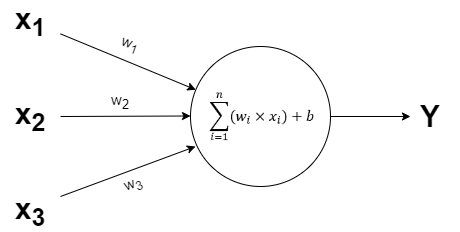
\includegraphics[width=0.5\textwidth]{Images/perceptron.png}
    \caption{Perceptron}
    \label{fig:Perceptron}
  \end{figure}

\subsection{Multi-layer Perceptron}
Neural networks are constructed by interconnecting multiple layers of neurons, integrating non-linear activation functions such as sigmoid and ReLU between these layers (Figure \ref{fig:activation}) \cite{activation}. The process of computing the output from this composite function for a given input is termed Forward Propagation.
\begin{figure}[h]
    \centering
    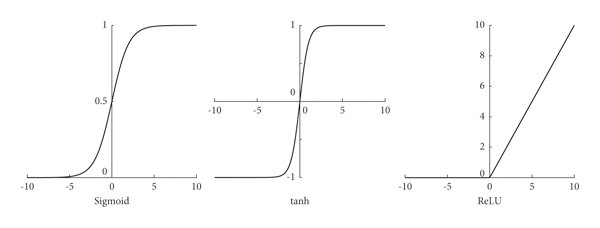
\includegraphics[width=1\textwidth]{Images/activation.png}
    \caption{Non-linear activation functions - a) Sigmoid b) tanh c) ReLU}
    \label{fig:activation}
  \end{figure}
Neural networks, as universal approximators which efficiently approximate nearly any continuous function. The incorporation of multiple layers of neurons and activation functions enables them with the ability to approximate intricate functions. The weights and biases associated with the neurons initiated randomly and learned during training. Figure \ref{fig:mlp} illustrates a two-layered network).
\begin{figure}[h]
    \centering
    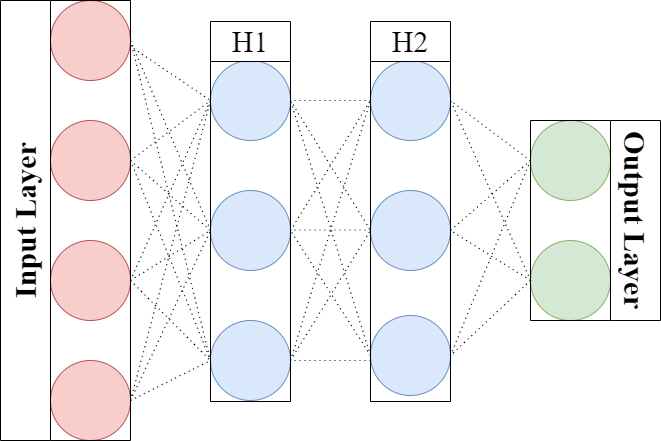
\includegraphics[width=0.5\textwidth]{Images/mlp.png}
    \caption{Fully connected network with 2 hidden layer}
    \label{fig:mlp}
  \end{figure}
Mathematically, the network function is represented as a probabilistic function, with the output \(Y\) expressed as \(p(y|x)\).
\subsection{Loss Functions}
Loss functions, also termed cost functions, evaluate the deviation between the original and predicted data points. These metrics guide network training towards minimizing this deviation. Popular loss functions include Mean Square Error, Entropy loss, and KL divergence. The loss function is selected based on the data and specific use case.
\subsection{Optimizers}
Optimizers represent the methods used in neural network training. They facilitate learning the network's parameters (weights and biases) to minimize the network's cost function. Usually, this is achieved by computing parameter gradients with respect to the loss function and updating these parameters by a step size in a manner that shifts their gradients towards the global minimum:

\[P_{\text{new}} = P_{\text{old}} - \alpha \nabla L(P_{\text{old}})\]

Here, \(\nabla L(P_{\text{old}})\) denotes the gradient of the loss function with respect to \(P_{\text{old}}\). Typically, in multi-layered networks, parameter gradients are calculated using the chain rule. The learning rate (\(\alpha\)) signifies the speed of parameter updates, often diminished during training, to prevent skipping the minimum. This iterative parameter update process called as Backpropagation. Various optimization techniques such as RMSprop, ADAM, Adagrad, and Adadelta are used in neural network training.

\subsection{Training}
The training process includes iteratively backpropagating through the network until the loss is minimized and stabilizes. Segmentation of the training data into batches enhances computational efficiency and expedites training. The backpropagation across all batches in the training data constitutes an epoch. Metrics like accuracy, monitor the training progress. Furthermore, a small set of training data which are not utilized for training, is employed to validate the model during the training.

\subsection{Batch Normalization}
Batch normalization is a technique in neural networks, optimizing the training process by normalizing layer inputs within mini-batches. Computation of batch-wise mean and variance enables normalization of inputs, resulting in faster convergence, mitigating vanishing or exploding gradients, and reducing sensitivity to weight initialization.


\section{Generative AI}
Generative AI represents a domain uses artificial intelligence concepts to generate novel data instances. Initially, Various machine learning methods such as deep learning are used for classification and prediction. However, over the years these models have evolved to create data instances. Trained to learn the density of distributions within the training data, these models include various architectures tailored to specific data. For instance, Convolutional Neural Networks performs well in learning patterns and features within images, while Recurrent Neural Networks proficiently learn temporal relationships in data sequences.


Once the model learned the distribution of the training data, these models possess the capability to generate new data points by sampling from the learned distribution. These generated data points typically diverge from the training corpus, yet effectively trained generative models exhibit the ability to generate data resembling the features found in the training data. This versatile methodology spans diverse fields, including image, music, and text generation. Generative modelling, based on learning the density of data distribution, categorized into two categories: Implicit and Explicit Density Models.

\paragraph*{Explicit Density Models}:
Explicit Density Models explicitly learn and estimate the probability distribution of input data. Variational Autoencoders (VAEs) and traditional probabilistic models is a typical example of this approach by explicitly modelling the probability distribution within a defined space. VAEs acquire a probabilistic representation of the data, enabling the generation of new samples through sampling from this learned distribution.

\paragraph*{Implicit Density Models}:
In contrast, Implicit Density Models do not explicitly define the probability distribution. Instead, they focus on generating new data points without directly modelling the probability distribution. Generative Adversarial Networks (GANs) fall in this category. GANs employ a generator network tasked with creating samples without explicitly defining the underlying probability distribution. The generator's objective is to generate data indistinguishable from real data, without directly modelling of the probability distribution.

The introduction of Generative Adversarial Networks in 2014 by Goodfellow et al \cite{7_gan}. marked a pivotal breakthrough in Generative AI. Initially applied for image generation, GANs stood out for producing high-quality images in contrast to the blurry images generated by VAEs. Early challenges such as Mode failure and training instability were addressed in subsequent GAN variants, solidifying its prominence in the domain. These models exhibit versatility across various data types such as videos, audios, signals…

The capacity to generate diverse and high-quality data finds various applications. In a proposed approach, these generated data drive a simulator used for training autonomous vehicles. Effective training of an Autonomous vehicle demands exposure to diverse scenarios, which existing simulators might limit. In this proposed methodology, a neural network model drives the simulator, generating requisite sensory data for autonomous vehicle training. This approach facilitates training the driving model on diverse scenarios, augmenting the vehicle's ability to generalize across various environments.

\section{Training data}
The training of a machine learning model in supervised setup, particularly in the domain of generative deep learning, heavily relies on data. The model's performance scales proportionally with the volume of training data on which it is trained on.

In this research, the synthesis of sensory data of autonomous vehicles alongside corresponding action labels proves challenging to obtain in substantial quantities from existing open-source datasets. While datasets like \cite{18_Waymo}, \cite{19_audi}, \cite{20_cityscapes} and \cite{21_panda} provide comprehensive sensory data at each time step, they lack the corresponding action labels.

Addressing this challenge, this research synthesizes data derived from a simulator, incorporating action labels. The generated data is rooted in the mathematical model of a 2D Lidar sensor installed on a vehicle navigating within a confined environment. Each instance in the dataset comprises (Observation at time step \(t\), action label, Observation at time step \(t+1\)). A dataset consisting of 150,000 such data points is generated and used to train the generative model. The anticipated outcome is the generation of new data points closely resembling those produced within the simulator environment.

\subsection{Mathematical Model-based Simulator}

The simulator is constructed using Python, featuring an environment mapped to the floor plan of our university building. The walls in the floor plan are represented as lines within the simulator, defined by their endpoint coordinates. A virtual vehicle navigating this environment is represented by a rectangular box scaled in accordance with the global environment boundaries. Simulated changes in the vehicle's position and orientation are executed by updating the vehicle boundary coordinates based on action commands.

The action command is formulated as a three-dimensional vector which includes the vehicle's velocity, turn angle, and turn direction. Vehicle velocity ranges between -5 to 5 units, while turn angle confined within 60 degrees on either side. The simulated 2D Lidar, mimicking observations from the vehicle, comprises a 360-sized vector. Each vector entry signifies the distance between the sensor and the closest obstacle around the vehicle for a given angle (360 degrees). This distance calculation entails projecting lines at each angle and checking for intersection with the environment's walls. The Cramer rule facilitates identifying intersection points between angle lines and wall lines, enabling the determination of closest distances of the obstacles from the vehicle. This iterative process across 360 degrees yields the observation at given timestep. Refer to Figure \ref{fig:simu} illustrating the vehicle, its projection lines, and the walls within the simulator. 
\begin{figure}[h]
    \centering
    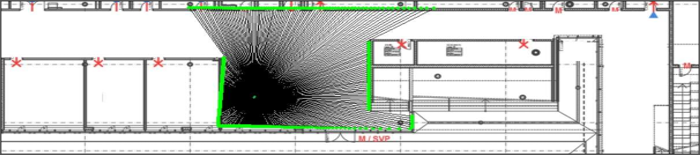
\includegraphics[width=0.80\textwidth]{Images/simu.png}
    \caption{Observation of the environment within the simulator}
    \label{fig:simu}
  \end{figure}

Successive sensor data calculated across two time steps are stored as a tuple alongside the corresponding action command, constituting each data point: \((O_t, A_t, O_{t+1})\)
Figure \ref{fig:befaft} visualizes the data variation across two consecutive time steps. Gaussian noise is injected in the data to make it robust, and the vehicle initializes at a new location upon collision or crossing walls. Randomly logged data points across time steps are shuffled, culminating in the logging of 150,000 data points for further training the generative model.
\begin{figure}[h]
    \centering
    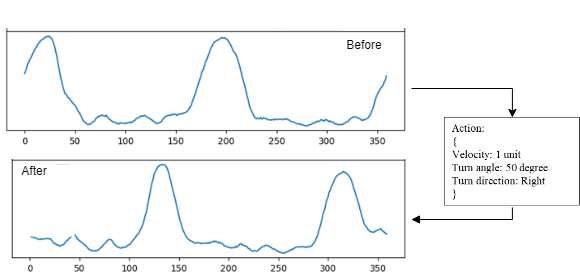
\includegraphics[width=1\textwidth]{Images/before after.png}
    \caption{Observations at two consecutive timesteps}
    \label{fig:befaft}
  \end{figure}

\section{Conditional Generative Adversarial Networks}
In Generative Adversarial Networks (GANs), the typical setup involves two models: the Generator \(G\) and the Discriminator \(D\). Traditionally, the generator \(G\) produces new instances \(y\) based on noise \(z\) sampled from a random distribution, and the generated data is represented as \(Y = G(z)\). However, this approach lacks control over the content of the generated data.

In this work, a conditional GAN architecture is employed, altering the generator's output to be conditioned on specific inputs—namely, the observation at the previous time step \(O_t\) and the action label \(A_t\). The Generator, in this context, generates the observation for the next time step based on the given previous timestep and action: \(O_{t+1} = G(O_t, A_t)\).

Conversely, the discriminator evaluates the conditional probability of the observation at the next time step \(O_{t+1}\) given \(O_t\) and \(A_t\):
\[D(O_t, O_{t+1}, A_t) = P(O_{t+1} | O_t, A_t)\]

This conditional setup allows for controlled generation of data, where the generator's output is influenced by inputs, leading to more tailored and context-aware generation.

\subsection{Generator}
The generator adopts an encoder-decoder architecture. Taking the previous timestep's sensor observation \(O_t\) and action label \(A_t\) as input, the encoder encodes the observation data into a 32-dimensional latent code. Simultaneously, the action label is passed through a Dense layer, and its output is concatenated with every layer of the encoder (refer to Figure \ref{fig:gen}). Additionally, a random 32-dimensional noise sampled from a normal distribution is passed through a linear layer and concatenated with the latent code, introducing noise for the generation of new objects within the output.

\begin{minipage}[t]{\linewidth}
        \centering
        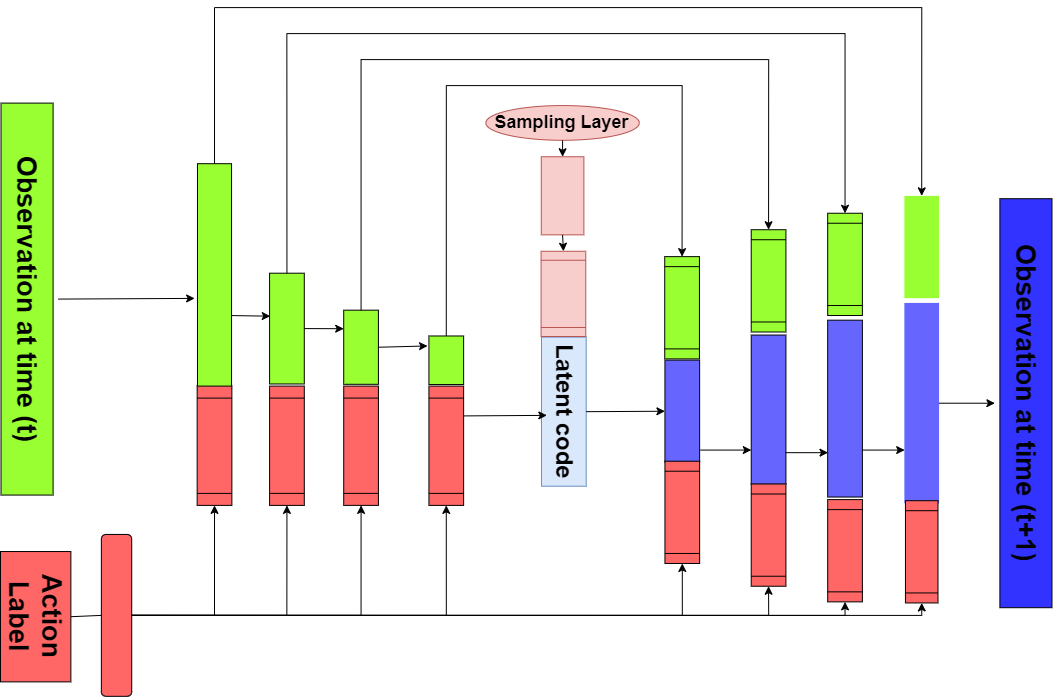
\includegraphics[width=1\textwidth]{Images/generator.png}
        \captionof{figure}{Generator Architecture}
        \label{fig:gen}
        \vspace{-\baselineskip} % Adjust spacing if needed
    \end{minipage}
    \hfill
  

The decoder accepts the latent code and random noise as input, producing the observation for the next timestep \(O_{gt+1}\) as output. Comprising four fully connected layers, each layer is concatenated with the action label and the output of the corresponding encoder layer (see Figure \ref{fig:gen}). By implementing these skip connections, information from the inputs is preserved after passing through the bottleneck. ReLU activation functions and batch normalization follow each layer in both the encoder and decoder.

\subsection{Discriminator}
The discriminator is a fully connected network processing three inputs: observation at timestep \(t\) \(O_t\), observation at timestep \(t+1\) \(O_{t+1}\), and the action label \(A_t\),. Both observations propagate forward through the network, while the action label undergoes pass via a dense layer and is concatenated with every layer in the network. The output layer consists of a single neuron with a sigmoid activation function (Figure \ref{fig:disc}). This network outputs the probability that the given observation pair concerning the action label is real. Furthermore, the network evaluates the authenticity of generated data.

\begin{minipage}[t]{\linewidth}
        \centering
        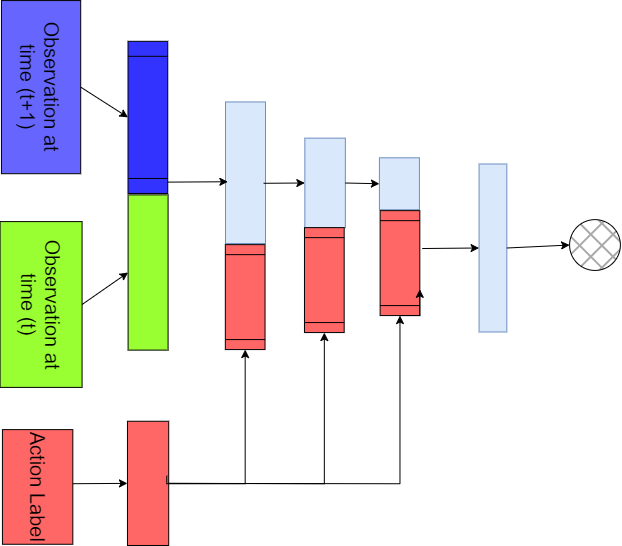
\includegraphics[width=0.5\textwidth]{Images/discriminator.png}
        \captionof{figure}{Discriminator Architecture}
        \label{fig:disc}
        \vspace{-\baselineskip} % Adjust spacing if needed
    \end{minipage}
    \hfill
  
\subsection{Training Loop}
The GAN's training occurs in two distinct steps: the individual training of the Generator and the Discriminator. A batch of data is fetched from the training corpus. The observation at the previous time step \(O_t\) and action label \(A_t\) are propagated through the generator, resulting in the generated observation for the next timestep \(O_{gt+1}\). This output, combined with generator inputs \((O_t, A_t)\), is then fed into the discriminator. The discriminator evaluates the probability of the authenticity of \(O_{gt+1}\) for given \(O_t\) and \(A_t\). Generated observations are assigned a 'fake' label ('0'), prompting computation of cross-entropy loss between these labels and the discriminator output. Additionally, mean square error is calculated between the generated observation \(O_{gt+1}\) and the actual observation \(O_{t+1}\). The generator gradients are computed with respect to the combined weighted loss, as expressed in the equation, and the generator gradients are updated:

\[Generator\ loss, L_g = L_d + \alpha \times MSE\]

For the discriminator, actual data \((O_t, O_{t+1}, A_t)\) is utilized, compared against the 'real' label ('1'). The sum of discriminator loss from both generated and actual data is calculated. Subsequently, the discriminator gradients are computed and updated concerning this combined discriminator loss:

\[Discriminator\ Loss = L_d\ real + L_d\ Generated\]

During generator training, discriminator weights are frozen, and vice versa, preventing either component from becoming overpowering. This alternating training of the generator and discriminator occurs for each epoch, facilitated by the use of the ADAM optimizer at adaptive learning rate
\chapter{Results and Discussions}
\section{Comparative metrics study}
The methodology proposed for assessing simulator suitability necessitates inputs from both simulator developers and users to validate the applicability of the derived scores. While the base score of simulators for proposed parameters can mostly be populated from official documentation, subjective parameters like "Photorealism" require alternative evaluation methods. To assess such subjective parameters, a collective perspective was gathered from various individuals. This included an average evaluation from multiple sources to ensure a well-rounded perspective. 
To assess user weights, two distinct user personas were identified, each with unique use cases for simulator:
\paragraph*{User 1: }  An University primarily focused on sensory data, feedback, and training deep learning models for projects. While realism holds importance, it's not a primary criterion.
\paragraph*{User 2: } A software tester at an automobile company dedicated to real-world model performance validation.
\paragraph*{User 3: } A research scholar dedicated to achieving autonomous driving within a confined environment, endeavoring to recreate customized real-world scenarios within the simulator.
\paragraph*{User 4: } Emphasizes extensive data generation, resembling a substantial data collector assembling datasets for various purposes, extending beyond autonomous driving or machine learning tasks.

Three simulators CARLA \cite{Carla}, Summit \cite{SUMMIT}, and LGVSL \cite{lgsvl} were considered for evaluation, with their base scores sourced from official documentation (Appendix).

The derived user weights for the identified personas (found in the appendix) were utilized to calculate final scores, summarized in Table \ref{tab:score}:
\begin{table}[H]
\centering
\renewcommand{\arraystretch}{1.5} % Adjust the vertical spacing in the table
\begin{tabular}{|p{2.5cm}|p{2.5cm}|p{2.5cm}|p{2.5cm}|} % Adjust the width of columns as needed
\hline
       & CARLA & Summit & LGVSL \\
\hline
User 1 & 18.5  & 21     & 19.7  \\
User 2 & 22.5  & 34     & 36    \\
User 3 & 16.65 &23.4    &22.4 \\
User 4 & 18.4  &29.2    &29.7\\
\hline
\end{tabular}
\caption{Final scores of comparisons}
\label{tab:score}
\end{table}


Interpreting the results, LGVSL emerges as a suitable choice for User 2, emphasizing the integration of real-world components, an essential criterion for their use case. Conversely, Summit resonates with User 1 due to its adeptness in simulating realistic traffic behaviours and leveraging CARLA's platform for training ML algorithms. 
A critical suggestion for refinement involves the introduction of a “mandatory parameter” criterion. This criterion would empower users to define indispensable parameters, and if a simulator under evaluation fails to offer them, it should be excluded from the assessment. This approach ensures that users can establish essential criteria tailored to their specific needs.
This comparative analysis showcases the varied suitability of simulators based on distinct user perspectives, emphasizing the importance of tailored assessments for specific use cases.

\section{Generative Model-Based Simulators}
The proposed architecture underwent training for 50 epochs utilizing a mini-batch size of 16. Figure \ref{fig:loss} illustrates the dynamic trends in generator and discriminator loss during the training phase.

\begin{minipage}[t]{\linewidth}
        \centering
        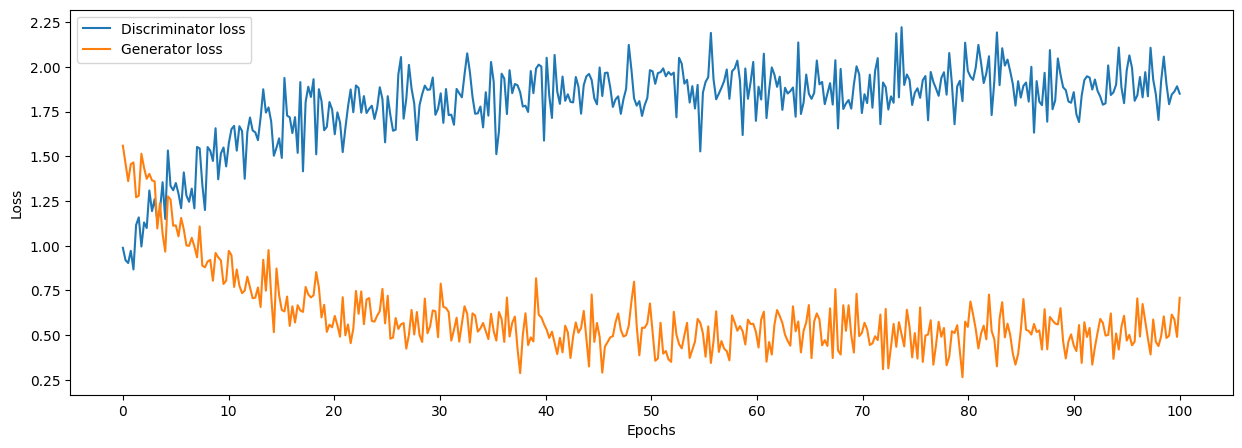
\includegraphics[width=1\textwidth]{Images/loss.png}
        \captionof{figure}{Generator and Discriminator Loss}
        \label{fig:loss}
        \vspace{-\baselineskip} % Adjust spacing if needed
    \end{minipage}
    \hfill

To optimize learning, the mean square loss weight parameter alpha was systematically reduced by half every 10 epochs. This strategy allowed the generator to initially focus on data reconstruction, progressively advancing to generate novel features.

Performance evaluation of the model involved rigorous testing with various customized action commands. Figure \ref{fig:trans} portrays the generation of subsequent observation $O_{g(t+1)}$ based on randomly chosen action vectors at a preceding time step ($O_{t}$).

\begin{minipage}[t]{\linewidth}
        \centering
        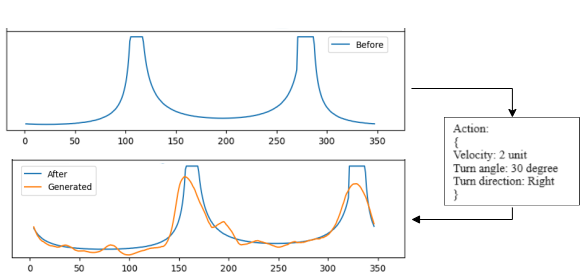
\includegraphics[width=1\textwidth]{Images/act_trans.png}
        \captionof{figure}[Transition of Observation for the Action Command]{Transition of Observation for the Action Command \textit{{Turn angle: 30 degrees, Turn direction: Right, Velocity: 2 units}}}
        \label{fig:trans}
        \vspace{-\baselineskip} % Adjust spacing if needed
    \end{minipage}
    \hfill

Evident shifts within the signal patterns validate the successful transition of observations in concordance with the designated action commands. Figure \ref{fig:trans} provides a comparative analysis between the generated output and the expected output for identical action commands.
While the generated output exhibited discernible noise and lacked the pristine quality of target output from the training corpus, no instances of new object generation were identified within the input.
The failure to generate new objects can be attributed to the limited diversity of objects within the training dataset. Furthermore, visually discerning the generation of plausible new objects within 2D lidar data posed significant challenges.
Recursive generation of outputs, wherein the generated output $O_{g(t+1)}$ serves as input for subsequent time steps, led to a cumulative increase in noise. Subsequently, this cumulative noise adversely impacted the fidelity of the environment's representation over time, as depicted in Figure \ref{fig:recout}, displaying observations generated recursively for 10 time steps.

\begin{minipage}[t]{\linewidth}
        \centering
        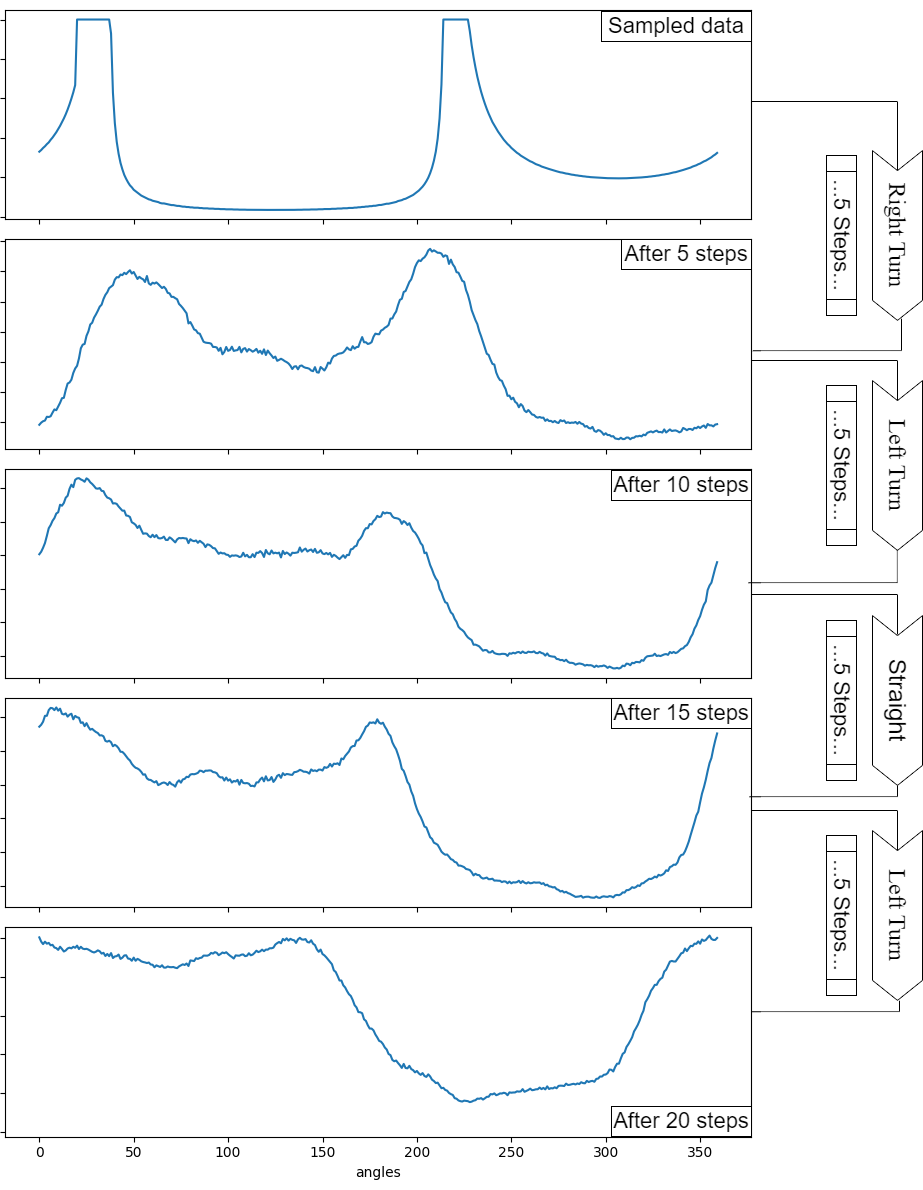
\includegraphics[width=0.9\textwidth]{Images/recout.png}
        \captionof{figure}{Recursive Generation of Sensor Observations}
        \label{fig:recout}
        \vspace{-\baselineskip} % Adjust spacing if needed
    \end{minipage}
    \hfill

Initial outputs exhibited commendable quality; however, the quality notably degraded after 5 steps.

\chapter{Conclusion}
This research includes two primary phases. The first segment aimed to establish a unified metric for evaluating the useability of diverse autonomous vehicle simulators. The objective was to quantify a simulator's usability based on user-specific requirements. An extensive study of available simulators and their respective use cases led to the identification of 73 distinct parameters for comparing these platforms. A scoring system was devised, allowing each parameter to be rated on a scale of 0 to 1.

The scoring system comprises two sets of scores: one assesses the simulator's capabilities (referred to as the Base score), while the other measures the significance of each parameter for a user and their intended application (referred to as user weight). The final score results from the combination of these two sets, offering a comprehensive representation of both simulator capability and user preferences. These final scores, generated for different evaluated simulators, serve as a basis for informed decision-making. A higher score signifies a better fit for the user's needs, facilitating a systematic comparison among various autonomous driving simulators. This approach streamlines the process of evaluating simulators, significantly reducing the time users spend navigating through documentation, installing simulators, and assessing their applicability. Moreover, it enables the creation of a precise overview of a simulator's functionalities.

The second segment of the thesis concentrated on developing a prototype simulator driven by a deep generative model. This approach aimed to replicate two fundamental functionalities of an autonomous driving simulator. Firstly, it focused on simulating the progression of sensory data to a subsequent state based on the executed action. Secondly, it aimed at generating a spectrum of novel scenarios crucial for training machine learning models to ensure their ability to generalize effectively.

The generative model's output was proposed to drive the simulator iteratively by using its own generated output as subsequent input in consecutive time steps. The scenario generation holds potential in aiding algorithms trained on this simulator to generalize more effectively, potentially addressing the issue of limited environmental diversity observed in certain simulators like Carla \cite{Carla}.

A conditional generative adversarial network was devised and trained using data obtained from a mathematical model-based simulator. Specifically, the network was trained on sensor data derived from a simulated 2D Lidar. The objective was to learn the transition of sensor data across multiple time steps in accordance with an action command represented by a 3-dimensional vector (Turn angle, Turn direction, Velocity). Furthermore, the trained model was intended to generate instances of such data representing plausible new scenarios.

The results indicated that the model effectively learned the physics underlying sensor and effectively modelled their data transitions in response to input action commands. However, limitations surfaced as the generated data did not introduce new objects and their representations in the 2D Lidar map. This shortcoming might stem from the lack of diversity in the training data. Additionally, noise was observed in the generated data, presenting challenges in identification and assessing the realism of newly generated objects within the 2D Lidar signal.


\chapter{Future works}
Future works regarding the comparative metric includes the potential introduction of a system that mandates parameters which are utmost crucial to users. Such mandatory parameters would signify critical criteria, and simulators failing to meet these standards could be excluded from evaluation rather than receiving higher weights. Additionally, considering that base scores remain constant for a specific simulator version, pre-establishing a list of base scores for widely used simulators would streamline the application of this evaluation system, ensuring user-friendly implementation. Moreover, the inclusion of new parameters derived from user feedback and reviews could enrich the evaluation framework, enhancing its relevance and comprehensiveness over time.

Regarding sensory data generation, there are several areas that can be improved. The methodology employed for learning the transition of 2D Lidar sensor data concerning given action commands could be extended to encompass other sensors prevalent in autonomous driving systems. Specifically, this approach could be extrapolated to generate sequential images based on prior image time steps and their respective actions. Accumulating diverse datasets across various scenarios could facilitate learning its distributions and the generation of diverse scenarios with novel objects integrated into the generated images. Evaluating and quantifying the realism of generated output is comparatively more straightforward in images than in Lidar data. Moreover, integrating specific filters such as low pass filters could diminish noise in the generated output (2D Lidar signals), preventing its accumulation across successive time steps. Training the model using datasets containing synchronized data from multiple sensors holds potential to enable the model to comprehend the correlations among sensors concerning their variations in response to actions, ultimately leading to the generation of synchronized multisensory data.


\backmatter
%%%%%%%%%%%%%%%%%%%
%% create figure list
%%%%%%%%%%%%%%%%%%%

\listoffigures

%%%%%%%%%%%%%%%%%%%
%% create tables list
%%%%%%%%%%%%%%%%%%%
\listoftables
%%%%%%%%%%%%%%%%%%%
%% create appendix
%%%%%%%%%%%%%%%%%%%
\setcounter{chapter}{1}
\renewcommand{\thechapter}{\Alph{chapter}}
\chapter*{Appendix}\label{appendix}
\addcontentsline{toc}{chapter}{Appendix}
The table \ref{tab:basescore} shows the scores of CARLA\cite{carla-docs}, SUMMIT \cite{summit-docs}, and LGVSL\cite{lgvsl-docs} simulators for each criterion in the proposed system for comparison. These scores are calculated based on the information from the official websites and documentation of the software.

\begin{longtable}[]{@{}
  >{\raggedright\arraybackslash}p{(\columnwidth - 12\tabcolsep) * \real{0.0478}}
  >{\raggedright\arraybackslash}p{(\columnwidth - 12\tabcolsep) * \real{0.0637}}
  >{\raggedright\arraybackslash}p{(\columnwidth - 12\tabcolsep) * \real{0.2767}}
  >{\raggedright\arraybackslash}p{(\columnwidth - 12\tabcolsep) * \real{0.2138}}
  >{\raggedright\arraybackslash}p{(\columnwidth - 12\tabcolsep) * \real{0.1315}}
  >{\raggedright\arraybackslash}p{(\columnwidth - 12\tabcolsep) * \real{0.1396}}
  >{\raggedright\arraybackslash}p{(\columnwidth - 12\tabcolsep) * \real{0.1270}}@{}}
\toprule()
\multicolumn{4}{@{}>{\raggedright\arraybackslash}p{(\columnwidth - 12\tabcolsep) * \real{0.6019} + 6\tabcolsep}}{%
\begin{minipage}[b]{\linewidth}\raggedright
\end{minipage}} & \begin{minipage}[b]{\linewidth}\raggedright
CARLA
\end{minipage} & \begin{minipage}[b]{\linewidth}\raggedright
SUMMIT
\end{minipage} & \begin{minipage}[b]{\linewidth}\raggedright
LGVSL
\end{minipage} \\
\midrule()
\endhead
\multicolumn{4}{@{}>{\raggedright\arraybackslash}p{(\columnwidth - 12\tabcolsep) * \real{0.6019} + 6\tabcolsep}}{%
1. Sensors} & & & \\
\hline


\multirow{16}{*}{a} &
\multicolumn{3}{>{\raggedright\arraybackslash}p{(\columnwidth - 12\tabcolsep) * \real{0.5541} + 4\tabcolsep}}{%
Ready to use Sensor} & & & \\
& i &
\multicolumn{2}{>{\raggedright\arraybackslash}p{(\columnwidth - 12\tabcolsep) * \real{0.4905} + 2\tabcolsep}}{%
RGB Camera} & 1 & 1 & 1 \\
& ii &
\multicolumn{2}{>{\raggedright\arraybackslash}p{(\columnwidth - 12\tabcolsep) * \real{0.4905} + 2\tabcolsep}}{%
Depth Camera} & 1 & 1 & 0 \\
& iii &
\multicolumn{2}{>{\raggedright\arraybackslash}p{(\columnwidth - 12\tabcolsep) * \real{0.4905} + 2\tabcolsep}}{%
3D Lidar} & 0 & 0 & 1 \\
& iv &
\multicolumn{2}{>{\raggedright\arraybackslash}p{(\columnwidth - 12\tabcolsep) * \real{0.4905} + 2\tabcolsep}}{%
Radar} & 1 & 1 & 1 \\
& v &
\multicolumn{2}{>{\raggedright\arraybackslash}p{(\columnwidth - 12\tabcolsep) * \real{0.4905} + 2\tabcolsep}}{%
IMU Sensor} & 1 & 1 & 1 \\
& vi &
\multicolumn{2}{>{\raggedright\arraybackslash}p{(\columnwidth - 12\tabcolsep) * \real{0.4905} + 2\tabcolsep}}{%
Semantic info Sensor} & 1 & 1 & 1 \\
& vii &
\multicolumn{2}{>{\raggedright\arraybackslash}p{(\columnwidth - 12\tabcolsep) * \real{0.4905} + 2\tabcolsep}}{%
Force Impact Sensor} & 0 & 1 & 1 \\
& viii &
\multicolumn{2}{>{\raggedright\arraybackslash}p{(\columnwidth - 12\tabcolsep) * \real{0.4905} + 2\tabcolsep}}{%
Lane detection/ infringement sensor} & 1 & 1 & 0 \\
& ix &
\multicolumn{2}{>{\raggedright\arraybackslash}p{(\columnwidth - 12\tabcolsep) * \real{0.4905} + 2\tabcolsep}}{%
Fuel/ Battery sensor} & 0 & 0 & 0 \\
& x &
\multicolumn{2}{>{\raggedright\arraybackslash}p{(\columnwidth - 12\tabcolsep) * \real{0.4905} + 2\tabcolsep}}{%
Vehicle speed sensor} & 0 & 1 & 1 \\
& xi &
\multicolumn{2}{>{\raggedright\arraybackslash}p{(\columnwidth - 12\tabcolsep) * \real{0.4905} + 2\tabcolsep}}{%
GPS} & 1 & 0 & 1 \\
& xii &
\multicolumn{2}{>{\raggedright\arraybackslash}p{(\columnwidth - 12\tabcolsep) * \real{0.4905} + 2\tabcolsep}}{%
Visiblity Sensor} & 0 & 0 & 0 \\
& xiii &
\multicolumn{2}{>{\raggedright\arraybackslash}p{(\columnwidth - 12\tabcolsep) * \real{0.4905} + 2\tabcolsep}}{%
Other vehicle sensors related to vehicle dynamics} & 0 & 0 & 0 \\
& xiv &
\multicolumn{2}{>{\raggedright\arraybackslash}p{(\columnwidth - 12\tabcolsep) * \real{0.4905} + 2\tabcolsep}}{%
Other environment sensors related to perception} & 1 & 0 & 1 \\
& Xv &
\multicolumn{2}{>{\raggedright\arraybackslash}p{(\columnwidth - 12\tabcolsep) * \real{0.4905} + 2\tabcolsep}}{%
Macroscopic Global Sensor} & 0 & 0 & 0 \\
b &
\multicolumn{3}{>{\raggedright\arraybackslash}p{(\columnwidth - 12\tabcolsep) * \real{0.5541} + 4\tabcolsep}}{%
Multiple Synchronous Sensors} & 1 & 1 & 1 \\
c &
\multicolumn{3}{>{\raggedright\arraybackslash}p{(\columnwidth - 12\tabcolsep) * \real{0.5541} + 4\tabcolsep}}{%
User defined position and orientation of sensors} & 1 & 1 & 1 \\
d &
\multicolumn{3}{>{\raggedright\arraybackslash}p{(\columnwidth - 12\tabcolsep) * \real{0.5541} + 4\tabcolsep}}{%
Precision of the Sensor readings} & 0 & 0 & 0 \\
e &
\multicolumn{3}{>{\raggedright\arraybackslash}p{(\columnwidth - 12\tabcolsep) * \real{0.5541} + 4\tabcolsep}}{%
Availability of real time sensor models} & 0 & 0 & 1 \\
f &
\multicolumn{3}{>{\raggedright\arraybackslash}p{(\columnwidth - 12\tabcolsep) * \real{0.5541} + 4\tabcolsep}}{%
User defined Sensors and Observers} & 0 & 0 & 1 \\
~ & ~ & ~ & ~ & & & \\
\hline

\multicolumn{4}{@{}>{\raggedright\arraybackslash}p{(\columnwidth - 12\tabcolsep) * \real{0.6019} + 6\tabcolsep}}{%
2. Actors} & & & \\
\hline
\multirow{8}{*}{a} &
\multicolumn{3}{>{\raggedright\arraybackslash}p{(\columnwidth - 12\tabcolsep) * \real{0.5541} + 4\tabcolsep}}{%
Geometry} & & & \\

& i &
\multicolumn{2}{>{\raggedright\arraybackslash}p{(\columnwidth - 12\tabcolsep) * \real{0.4905} + 2\tabcolsep}}{%
Pre defines Scenarios} & 1 & 1 & 1 \\
& ii &
\multicolumn{2}{>{\raggedright\arraybackslash}p{(\columnwidth - 12\tabcolsep) * \real{0.4905} + 2\tabcolsep}}{%
Predefines models for Actors} & 1 & 1 & 1 \\
& iii &
\multicolumn{2}{>{\raggedright\arraybackslash}p{(\columnwidth - 12\tabcolsep) * \real{0.4905} + 2\tabcolsep}}{%
User-Defined Actors} & 0 & 0 & 0 \\
& iv &
\multicolumn{2}{>{\raggedright\arraybackslash}p{(\columnwidth - 12\tabcolsep) * \real{0.4905} + 2\tabcolsep}}{%
No. of Actors and Spawning Location} & 1 & 0 & 0 \\
& v &
\multicolumn{2}{>{\raggedright\arraybackslash}p{(\columnwidth - 12\tabcolsep) * \real{0.4905} + 2\tabcolsep}}{%
Recreation of Real time models} & 0 & 0 & 1 \\
& vi &
\multicolumn{2}{>{\raggedright\arraybackslash}p{(\columnwidth - 12\tabcolsep) * \real{0.4905} + 2\tabcolsep}}{%
Path/ destination of Actors} & 0 & 1 & 0 \\
& vii &
\multicolumn{2}{>{\raggedright\arraybackslash}p{(\columnwidth - 12\tabcolsep) * \real{0.4905} + 2\tabcolsep}}{%
Context aware spawning} & 0 & 0 & 0 \\
\multirow{7}{*}{b} &
\multicolumn{3}{>{\raggedright\arraybackslash}p{(\columnwidth - 12\tabcolsep) * \real{0.5541} + 4\tabcolsep}}{%
Behaviour} & & & \\
& i &
\multicolumn{2}{>{\raggedright\arraybackslash}p{(\columnwidth - 12\tabcolsep) * \real{0.4905} + 2\tabcolsep}}{%
Pre defined Rules} & 1 & 1 & 1 \\
& ii &
\multicolumn{2}{>{\raggedright\arraybackslash}p{(\columnwidth - 12\tabcolsep) * \real{0.4905} + 2\tabcolsep}}{%
User defined Rules} & 0 & 1 & 1 \\
& iii &
\multicolumn{2}{>{\raggedright\arraybackslash}p{(\columnwidth - 12\tabcolsep) * \real{0.4905} + 2\tabcolsep}}{%
Distinguishable Behavioural pattern} & 0 & 1 & 0 \\
& iv &
\multicolumn{2}{>{\raggedright\arraybackslash}p{(\columnwidth - 12\tabcolsep) * \real{0.4905} + 2\tabcolsep}}{%
Sensitivity} & 1 & 1 & 1 \\
& v &
\multicolumn{2}{>{\raggedright\arraybackslash}p{(\columnwidth - 12\tabcolsep) * \real{0.4905} + 2\tabcolsep}}{%
Level of aggressiveness in driving} & 0 & 0 & 0 \\
& vi &
\multicolumn{2}{>{\raggedright\arraybackslash}p{(\columnwidth - 12\tabcolsep) * \real{0.4905} + 2\tabcolsep}}{%
Reproducibility} & 0 & 0 & 1 \\
~ & ~ & ~ & ~ & & & \\
\hline
\multicolumn{4}{@{}>{\raggedright\arraybackslash}p{(\columnwidth - 12\tabcolsep) * \real{0.6019} + 6\tabcolsep}}{%
3. Environment} & & & \\
\hline
a &
\multicolumn{3}{>{\raggedright\arraybackslash}p{(\columnwidth - 12\tabcolsep) * \real{0.5541} + 4\tabcolsep}}{%
Pre defined libraries} & 1 & 1 & 1 \\
b &
\multicolumn{3}{>{\raggedright\arraybackslash}p{(\columnwidth - 12\tabcolsep) * \real{0.5541} + 4\tabcolsep}}{%
User defined environments} & 0 & 1 & 1 \\
c &
\multicolumn{3}{>{\raggedright\arraybackslash}p{(\columnwidth - 12\tabcolsep) * \real{0.5541} + 4\tabcolsep}}{%
Real world maps} & 0 & 1 & 1 \\
d &
\multicolumn{3}{>{\raggedright\arraybackslash}p{(\columnwidth - 12\tabcolsep) * \real{0.5541} + 4\tabcolsep}}{%
Photorealism} & 0 & 1 & 1 \\
e &
\multicolumn{3}{>{\raggedright\arraybackslash}p{(\columnwidth - 12\tabcolsep) * \real{0.5541} + 4\tabcolsep}}{%
Variable resolution} & 0 & 0 & 0 \\
f &
\multicolumn{3}{>{\raggedright\arraybackslash}p{(\columnwidth - 12\tabcolsep) * \real{0.5541} + 4\tabcolsep}}{%
Context aware map-planning} & 0 & 1 & 0 \\
g &
\multicolumn{3}{>{\raggedright\arraybackslash}p{(\columnwidth - 12\tabcolsep) * \real{0.5541} + 4\tabcolsep}}{%
User defined scenarios} & 0 & 1 & 1 \\
h &
\multicolumn{3}{>{\raggedright\arraybackslash}p{(\columnwidth - 12\tabcolsep) * \real{0.5541} + 4\tabcolsep}}{%
Material defenition} & 0 & 0 & 1 \\
i &
\multicolumn{3}{>{\raggedright\arraybackslash}p{(\columnwidth - 12\tabcolsep) * \real{0.5541} + 4\tabcolsep}}{%
Variable levels of sun shades} & 1 & 1 & 1 \\
j &
\multicolumn{3}{>{\raggedright\arraybackslash}p{(\columnwidth - 12\tabcolsep) * \real{0.5541} + 4\tabcolsep}}{%
Special optical feautres} & 0 & 0 & 1 \\
k &
\multicolumn{3}{>{\raggedright\arraybackslash}p{(\columnwidth - 12\tabcolsep) * \real{0.5541} + 4\tabcolsep}}{%
Data visualization and analytical tools} & 0 & 1 & 1 \\
l &
\multicolumn{3}{>{\raggedright\arraybackslash}p{(\columnwidth - 12\tabcolsep) * \real{0.5541} + 4\tabcolsep}}{%
Rendering} & 0 & 1 & 1 \\
m &
\multicolumn{3}{>{\raggedright\arraybackslash}p{(\columnwidth - 12\tabcolsep) * \real{0.5541} + 4\tabcolsep}}{%
Recording} & 0 & 1 & 1 \\
~ & ~ & ~ & ~ & & & \\
\hline

\multicolumn{4}{@{}>{\raggedright\arraybackslash}p{(\columnwidth - 12\tabcolsep) * \real{0.6019} + 6\tabcolsep}}{%
4. Ego Vehicle} & & & \\
\hline

a &
\multicolumn{3}{>{\raggedright\arraybackslash}p{(\columnwidth - 12\tabcolsep) * \real{0.5541} + 4\tabcolsep}}{%
Vehicle Geometry} & 1 & 1 & 1 \\
b &
\multicolumn{3}{>{\raggedright\arraybackslash}p{(\columnwidth - 12\tabcolsep) * \real{0.5541} + 4\tabcolsep}}{%
Wheel Geometry} & 0 & 1 & 1 \\
c &
\multicolumn{3}{>{\raggedright\arraybackslash}p{(\columnwidth - 12\tabcolsep) * \real{0.5541} + 4\tabcolsep}}{%
Real world models} & 0 & 1 & 1 \\
d &
\multicolumn{3}{>{\raggedright\arraybackslash}p{(\columnwidth - 12\tabcolsep) * \real{0.5541} + 4\tabcolsep}}{%
Real world physics} & 0 & 1 & 1 \\
e &
\multicolumn{3}{>{\raggedright\arraybackslash}p{(\columnwidth - 12\tabcolsep) * \real{0.5541} + 4\tabcolsep}}{%
Input commands} & 1 & 1 & 1 \\
f &
\multicolumn{3}{>{\raggedright\arraybackslash}p{(\columnwidth - 12\tabcolsep) * \real{0.5541} + 4\tabcolsep}}{%
Other components} & 0 & 0 & 0 \\
~ & ~ & ~ & ~ & & & \\
\hline

\multicolumn{4}{@{}>{\raggedright\arraybackslash}p{(\columnwidth - 12\tabcolsep) * \real{0.6019} + 6\tabcolsep}}{%
5. Framework} & & & \\
\hline

a &
\multicolumn{3}{>{\raggedright\arraybackslash}p{(\columnwidth - 12\tabcolsep) * \real{0.5541} + 4\tabcolsep}}{%
Cross platform Compatability} & & & \\
~ & i &
\multicolumn{2}{>{\raggedright\arraybackslash}p{(\columnwidth - 12\tabcolsep) * \real{0.4905} + 2\tabcolsep}}{%
Linux} & 1 & 1 & 1 \\
~ & ii &
\multicolumn{2}{>{\raggedright\arraybackslash}p{(\columnwidth - 12\tabcolsep) * \real{0.4905} + 2\tabcolsep}}{%
ROS} & 1 & 0 & 1 \\
~ & iii &
\multicolumn{2}{>{\raggedright\arraybackslash}p{(\columnwidth - 12\tabcolsep) * \real{0.4905} + 2\tabcolsep}}{%
Windows} & 1 & 1 & 0 \\
~ & iv &
\multicolumn{2}{>{\raggedright\arraybackslash}p{(\columnwidth - 12\tabcolsep) * \real{0.4905} + 2\tabcolsep}}{%
MacOS} & 1 & 1 & 0 \\
~ & v &
\multicolumn{2}{>{\raggedright\arraybackslash}p{(\columnwidth - 12\tabcolsep) * \real{0.4905} + 2\tabcolsep}}{%
Other} & 1 & 0 & 0 \\
b &
\multicolumn{3}{>{\raggedright\arraybackslash}p{(\columnwidth - 12\tabcolsep) * \real{0.5541} + 4\tabcolsep}}{%
Open Source} & 1 & 1 & 0 \\
c &
\multicolumn{3}{>{\raggedright\arraybackslash}p{(\columnwidth - 12\tabcolsep) * \real{0.5541} + 4\tabcolsep}}{%
Scripting Language support} & & & \\
~ & i &
\multicolumn{2}{>{\raggedright\arraybackslash}p{(\columnwidth - 12\tabcolsep) * \real{0.4905} + 2\tabcolsep}}{%
Python} & 1 & 1 & 1 \\
~ & ii &
\multicolumn{2}{>{\raggedright\arraybackslash}p{(\columnwidth - 12\tabcolsep) * \real{0.4905} + 2\tabcolsep}}{%
C++} & 1 & 1 & 0 \\
~ & iii &
\multicolumn{2}{>{\raggedright\arraybackslash}p{(\columnwidth - 12\tabcolsep) * \real{0.4905} + 2\tabcolsep}}{%
R} & 0 & 0 & 0 \\
~ & iv &
\multicolumn{2}{>{\raggedright\arraybackslash}p{(\columnwidth - 12\tabcolsep) * \real{0.4905} + 2\tabcolsep}}{%
Java} & 0 & 0 & 0 \\
~ & v &
\multicolumn{2}{>{\raggedright\arraybackslash}p{(\columnwidth - 12\tabcolsep) * \real{0.4905} + 2\tabcolsep}}{%
Others} & 0 & 0 & 0 \\
d &
\multicolumn{3}{>{\raggedright\arraybackslash}p{(\columnwidth - 12\tabcolsep) * \real{0.5541} + 4\tabcolsep}}{%
Scalability} & 0 & 1 & 0 \\
e &
\multicolumn{3}{>{\raggedright\arraybackslash}p{(\columnwidth - 12\tabcolsep) * \real{0.5541} + 4\tabcolsep}}{%
Computation resource evaluation} & 0.5 & 0.5 & 0.7 \\
f &
\multicolumn{3}{>{\raggedright\arraybackslash}p{(\columnwidth - 12\tabcolsep) * \real{0.5541} + 4\tabcolsep}}{%
Community support} & & & \\
~ & i &
\multicolumn{2}{>{\raggedright\arraybackslash}p{(\columnwidth - 12\tabcolsep) * \real{0.4905} + 2\tabcolsep}}{%
Structured documentation} & 1 & 1 & 1 \\
~ & ii &
\multicolumn{2}{>{\raggedright\arraybackslash}p{(\columnwidth - 12\tabcolsep) * \real{0.4905} + 2\tabcolsep}}{%
Tutorials} & 1 & 1 & 0 \\
~ & iii &
\multicolumn{2}{>{\raggedright\arraybackslash}p{(\columnwidth - 12\tabcolsep) * \real{0.4905} + 2\tabcolsep}}{%
Discussion Forums} & 0 & 0 & 0 \\
g &
\multicolumn{3}{>{\raggedright\arraybackslash}p{(\columnwidth - 12\tabcolsep) * \real{0.5541} + 4\tabcolsep}}{%
Distributed Computing} & 1 & 0 & 0 \\
~ & ~ & ~ & ~ & & & \\
\hline

\multicolumn{4}{@{}>{\raggedright\arraybackslash}p{(\columnwidth - 12\tabcolsep) * \real{0.6019} + 6\tabcolsep}}{%
6. Driving Algorithm} & & & \\
\hline

a &
\multicolumn{3}{>{\raggedright\arraybackslash}p{(\columnwidth - 12\tabcolsep) * \real{0.5541} + 4\tabcolsep}}{%
Data Exchange} & 1 & 1 & 1 \\
b &
\multicolumn{3}{>{\raggedright\arraybackslash}p{(\columnwidth - 12\tabcolsep) * \real{0.5541} + 4\tabcolsep}}{%
Data Logging} & 1 & 1 & 0 \\
c &
\multicolumn{3}{>{\raggedright\arraybackslash}p{(\columnwidth - 12\tabcolsep) * \real{0.5541} + 4\tabcolsep}}{%
Hardware in Loop (HiL)} & 0 & 0 & 1 \\
d &
\multicolumn{3}{>{\raggedright\arraybackslash}p{(\columnwidth - 12\tabcolsep) * \real{0.5541} + 4\tabcolsep}}{%
ML Libraries} & 0 & 0 & 0 \\
\bottomrule()
\caption{Base Score for Carla, Summit. LGVSL} \label{tab:basescore} \\
\end{longtable}

The table displays the criteria weights provided by four distinct users within the comparison system. Here's a brief description of each user and their respective use case:
\textbf{User1: }A university student primarily focused on projects involving sensory data generation, feedback, and training deep learning models. While realism isn't a top priority, it would be advantageous.
\textbf{User2:} A software tester at an automobile company concentrating on validating model performance in real-world scenarios.
\textbf{User3:} A research scholar striving to achieve autonomous driving within a confined environment, aiming to replicate real-world custom environments within the simulator.
\textbf{User4:} Emphasizes extensive data generation, resembling a large-scale data collector preparing datasets for various tasks, not limited to autonomous driving or machine learning. Hence, customization options and distributed computing hold significant importance.


\begin{longtable}[]{@{}
  >{\raggedright\arraybackslash}p{(\columnwidth - 14\tabcolsep) * \real{0.0472}}
  >{\raggedright\arraybackslash}p{(\columnwidth - 14\tabcolsep) * \real{0.0602}}
  >{\raggedright\arraybackslash}p{(\columnwidth - 14\tabcolsep) * \real{0.1534}}
  >{\raggedright\arraybackslash}p{(\columnwidth - 14\tabcolsep) * \real{0.2946}}
  >{\raggedright\arraybackslash}p{(\columnwidth - 14\tabcolsep) * \real{0.1111}}
  >{\raggedright\arraybackslash}p{(\columnwidth - 14\tabcolsep) * \real{0.0952}}
  >{\raggedright\arraybackslash}p{(\columnwidth - 14\tabcolsep) * \real{0.1112}}
  >{\raggedright\arraybackslash}p{(\columnwidth - 14\tabcolsep) * \real{0.1270}}@{}}
\toprule()
\multicolumn{4}{@{}>{\raggedright\arraybackslash}p{(\columnwidth - 14\tabcolsep) * \real{0.5553} + 6\tabcolsep}}{%
\begin{minipage}[b]{\linewidth}\raggedright
\end{minipage}} & \begin{minipage}[b]{\linewidth}\raggedright
User 1
\end{minipage} & \begin{minipage}[b]{\linewidth}\raggedright
User 2
\end{minipage} & \begin{minipage}[b]{\linewidth}\raggedright
User 3
\end{minipage} & \begin{minipage}[b]{\linewidth}\raggedright
User 4
\end{minipage} \\
\midrule()
\endhead
\multicolumn{4}{@{}>{\raggedright\arraybackslash}p{(\columnwidth - 14\tabcolsep) * \real{0.5553} + 6\tabcolsep}}{%
1. Sensors} & & & & \\
\hline

\multirow{16}{*}{a} &
\multicolumn{3}{>{\raggedright\arraybackslash}p{(\columnwidth - 14\tabcolsep) * \real{0.5082} + 4\tabcolsep}}{%
Ready to use Sensor} & & & & \\
& i &
\multicolumn{2}{>{\raggedright\arraybackslash}p{(\columnwidth - 14\tabcolsep) * \real{0.4480} + 2\tabcolsep}}{%
RGB Camera} & 0 & 1 & 1 & 0.6 \\
& ii &
\multicolumn{2}{>{\raggedright\arraybackslash}p{(\columnwidth - 14\tabcolsep) * \real{0.4480} + 2\tabcolsep}}{%
Depth Camera} & 1 & 1 & 0.5 & 1 \\
& iii &
\multicolumn{2}{>{\raggedright\arraybackslash}p{(\columnwidth - 14\tabcolsep) * \real{0.4480} + 2\tabcolsep}}{%
3D Lidar} & 0 & 1 & 1 & 1 \\
& iv &
\multicolumn{2}{>{\raggedright\arraybackslash}p{(\columnwidth - 14\tabcolsep) * \real{0.4480} + 2\tabcolsep}}{%
Radar} & 0 & 0 & 0.7 & 1 \\
& v &
\multicolumn{2}{>{\raggedright\arraybackslash}p{(\columnwidth - 14\tabcolsep) * \real{0.4480} + 2\tabcolsep}}{%
IMU Sensor} & 0 & 1 & 0.5 & 1 \\
& vi &
\multicolumn{2}{>{\raggedright\arraybackslash}p{(\columnwidth - 14\tabcolsep) * \real{0.4480} + 2\tabcolsep}}{%
Semantic info Sensor} & 1 & 0 & 0.5 & 0.6 \\
& vii &
\multicolumn{2}{>{\raggedright\arraybackslash}p{(\columnwidth - 14\tabcolsep) * \real{0.4480} + 2\tabcolsep}}{%
Force Impact Sensor} & 0 & 1 & 0 & 1 \\
& viii &
\multicolumn{2}{>{\raggedright\arraybackslash}p{(\columnwidth - 14\tabcolsep) * \real{0.4480} + 2\tabcolsep}}{%
Lane detection/ infringement sensor} & 1 & 1 & 0.1 & 1 \\
& ix &
\multicolumn{2}{>{\raggedright\arraybackslash}p{(\columnwidth - 14\tabcolsep) * \real{0.4480} + 2\tabcolsep}}{%
Fuel/ Battery sensor} & 0 & 1 & 1 & 1 \\
& x &
\multicolumn{2}{>{\raggedright\arraybackslash}p{(\columnwidth - 14\tabcolsep) * \real{0.4480} + 2\tabcolsep}}{%
Vehicle speed sensor} & 0 & 1 & 1 & 1 \\
& xi &
\multicolumn{2}{>{\raggedright\arraybackslash}p{(\columnwidth - 14\tabcolsep) * \real{0.4480} + 2\tabcolsep}}{%
GPS} & 0 & 1 & 1 & 1 \\
& xii &
\multicolumn{2}{>{\raggedright\arraybackslash}p{(\columnwidth - 14\tabcolsep) * \real{0.4480} + 2\tabcolsep}}{%
Visiblity Sensor} & 0 & 0 & 0.1 & 0.6 \\
& xiii &
\multicolumn{2}{>{\raggedright\arraybackslash}p{(\columnwidth - 14\tabcolsep) * \real{0.4480} + 2\tabcolsep}}{%
Other vehicle sensors related to vehicle dynamics} & 0 & 1 & 0.3 &
0.6 \\
& xiv &
\multicolumn{2}{>{\raggedright\arraybackslash}p{(\columnwidth - 14\tabcolsep) * \real{0.4480} + 2\tabcolsep}}{%
Other environment sensors related to perception} & 1 & 0 & 0.2 & 0.5 \\
& Xv &
\multicolumn{2}{>{\raggedright\arraybackslash}p{(\columnwidth - 14\tabcolsep) * \real{0.4480} + 2\tabcolsep}}{%
Macroscopic Global Sensor} & 0 & 0 & 0.5 & 0.1 \\
b &
\multicolumn{3}{>{\raggedright\arraybackslash}p{(\columnwidth - 14\tabcolsep) * \real{0.5082} + 4\tabcolsep}}{%
Multiple Synchronous Sensors} & 1 & 1 & 1 & 1 \\
c &
\multicolumn{3}{>{\raggedright\arraybackslash}p{(\columnwidth - 14\tabcolsep) * \real{0.5082} + 4\tabcolsep}}{%
User defined position and orientation of sensors} & 0 & 1 & 1 & 1 \\
d &
\multicolumn{3}{>{\raggedright\arraybackslash}p{(\columnwidth - 14\tabcolsep) * \real{0.5082} + 4\tabcolsep}}{%
Precision of the Sensor readings} & 0 & 1 & 1 & 1 \\
e &
\multicolumn{3}{>{\raggedright\arraybackslash}p{(\columnwidth - 14\tabcolsep) * \real{0.5082} + 4\tabcolsep}}{%
Availability of real time sensor models} & 0 & 1 & 0.9 & 1 \\
f &
\multicolumn{3}{>{\raggedright\arraybackslash}p{(\columnwidth - 14\tabcolsep) * \real{0.5082} + 4\tabcolsep}}{%
User defined Sensors and Observers} & 1 & 0 & 0.5 & 0.9 \\
~ & ~ & ~ & ~ & & & & \\
\hline

\multicolumn{4}{@{}>{\raggedright\arraybackslash}p{(\columnwidth - 14\tabcolsep) * \real{0.5553} + 6\tabcolsep}}{%
2. Actors} & & & & \\
\hline

\multirow{8}{*}{a} &
\multicolumn{3}{>{\raggedright\arraybackslash}p{(\columnwidth - 14\tabcolsep) * \real{0.5082} + 4\tabcolsep}}{%
Geometry} & & & & \\
& i &
\multicolumn{2}{>{\raggedright\arraybackslash}p{(\columnwidth - 14\tabcolsep) * \real{0.4480} + 2\tabcolsep}}{%
Pre defines Scenarios} & 1 & 1 & 1 & 0.2 \\
& ii &
\multicolumn{2}{>{\raggedright\arraybackslash}p{(\columnwidth - 14\tabcolsep) * \real{0.4480} + 2\tabcolsep}}{%
Predefines models for Actors} & 1 & 1 & 1 & 0.6 \\
& iii &
\multicolumn{2}{>{\raggedright\arraybackslash}p{(\columnwidth - 14\tabcolsep) * \real{0.4480} + 2\tabcolsep}}{%
User-Defined Actors} & 0 & 1 & 0.7 & 1 \\
& iv &
\multicolumn{2}{>{\raggedright\arraybackslash}p{(\columnwidth - 14\tabcolsep) * \real{0.4480} + 2\tabcolsep}}{%
No. of Actors and Spawning Location} & 0 & 1 & 1 & 1 \\
& v &
\multicolumn{2}{>{\raggedright\arraybackslash}p{(\columnwidth - 14\tabcolsep) * \real{0.4480} + 2\tabcolsep}}{%
Recreation of Real time models} & 0 & 1 & 0.7 & 1 \\
& vi &
\multicolumn{2}{>{\raggedright\arraybackslash}p{(\columnwidth - 14\tabcolsep) * \real{0.4480} + 2\tabcolsep}}{%
Path/ destination of Actors} & 0 & 1 & 1 & 1 \\
& vii &
\multicolumn{2}{>{\raggedright\arraybackslash}p{(\columnwidth - 14\tabcolsep) * \real{0.4480} + 2\tabcolsep}}{%
Context aware spawning} & 0 & 1 & 1 & 0.6 \\
\multirow{7}{*}{b} &
\multicolumn{3}{>{\raggedright\arraybackslash}p{(\columnwidth - 14\tabcolsep) * \real{0.5082} + 4\tabcolsep}}{%
Behaviour} & & & & \\
& i &
\multicolumn{2}{>{\raggedright\arraybackslash}p{(\columnwidth - 14\tabcolsep) * \real{0.4480} + 2\tabcolsep}}{%
Pre defined Rules} & 0.5 & 1 & 1 & 0.6 \\
& ii &
\multicolumn{2}{>{\raggedright\arraybackslash}p{(\columnwidth - 14\tabcolsep) * \real{0.4480} + 2\tabcolsep}}{%
User defined Rules} & 0.5 & 1 & 1 & 1 \\
& iii &
\multicolumn{2}{>{\raggedright\arraybackslash}p{(\columnwidth - 14\tabcolsep) * \real{0.4480} + 2\tabcolsep}}{%
Distinguishable Behavioural pattern} & 0 & 1 & 0.1 & 0.6 \\
& iv &
\multicolumn{2}{>{\raggedright\arraybackslash}p{(\columnwidth - 14\tabcolsep) * \real{0.4480} + 2\tabcolsep}}{%
Sensitivity} & 0.5 & 1 & 0.3 & 0.3 \\
& v &
\multicolumn{2}{>{\raggedright\arraybackslash}p{(\columnwidth - 14\tabcolsep) * \real{0.4480} + 2\tabcolsep}}{%
Level of aggressiveness in driving} & 0 & 1 & 0.2 & 0.6 \\
& vi &
\multicolumn{2}{>{\raggedright\arraybackslash}p{(\columnwidth - 14\tabcolsep) * \real{0.4480} + 2\tabcolsep}}{%
Reproducibility} & 1 & 0 & 1 & 0.5 \\
~ & ~ & ~ & ~ & & & & \\
\hline
\multicolumn{4}{@{}>{\raggedright\arraybackslash}p{(\columnwidth - 14\tabcolsep) * \real{0.5553} + 6\tabcolsep}}{%
3. Environment} & & & & \\
\hline
a &
\multicolumn{3}{>{\raggedright\arraybackslash}p{(\columnwidth - 14\tabcolsep) * \real{0.5082} + 4\tabcolsep}}{%
Pre defined libraries} & 1 & 1 & 1 & 0.7 \\
b &
\multicolumn{3}{>{\raggedright\arraybackslash}p{(\columnwidth - 14\tabcolsep) * \real{0.5082} + 4\tabcolsep}}{%
User defined environments} & 0 & 0 & 1 & 1 \\
c &
\multicolumn{3}{>{\raggedright\arraybackslash}p{(\columnwidth - 14\tabcolsep) * \real{0.5082} + 4\tabcolsep}}{%
Real world maps} & 0 & 1 & 0.7 & 0.5 \\
d &
\multicolumn{3}{>{\raggedright\arraybackslash}p{(\columnwidth - 14\tabcolsep) * \real{0.5082} + 4\tabcolsep}}{%
Photorealism} & 0.5 & 1 & 0.5 & 0.9 \\
e &
\multicolumn{3}{>{\raggedright\arraybackslash}p{(\columnwidth - 14\tabcolsep) * \real{0.5082} + 4\tabcolsep}}{%
Variable resolution} & 0 & 0 & 0.6 & 0.6 \\
f &
\multicolumn{3}{>{\raggedright\arraybackslash}p{(\columnwidth - 14\tabcolsep) * \real{0.5082} + 4\tabcolsep}}{%
Context aware map-planning} & 0 & 1 & 0.4 & 0.9 \\
g &
\multicolumn{3}{>{\raggedright\arraybackslash}p{(\columnwidth - 14\tabcolsep) * \real{0.5082} + 4\tabcolsep}}{%
User defined scenarios} & 1 & 1 & 0.7 & 1 \\
h &
\multicolumn{3}{>{\raggedright\arraybackslash}p{(\columnwidth - 14\tabcolsep) * \real{0.5082} + 4\tabcolsep}}{%
Material defenition} & 0 & 0.5 & 0.2 & 0.8 \\
i &
\multicolumn{3}{>{\raggedright\arraybackslash}p{(\columnwidth - 14\tabcolsep) * \real{0.5082} + 4\tabcolsep}}{%
Variable levels of sun shades} & 0 & 1 & 0.6 & 1 \\
j &
\multicolumn{3}{>{\raggedright\arraybackslash}p{(\columnwidth - 14\tabcolsep) * \real{0.5082} + 4\tabcolsep}}{%
Special optical feautres} & 0 & 1 & 0.1 & 0.7 \\
k &
\multicolumn{3}{>{\raggedright\arraybackslash}p{(\columnwidth - 14\tabcolsep) * \real{0.5082} + 4\tabcolsep}}{%
Data visualization and analytical tools} & 1 & 1 & 0.6 & 0.5 \\
l &
\multicolumn{3}{>{\raggedright\arraybackslash}p{(\columnwidth - 14\tabcolsep) * \real{0.5082} + 4\tabcolsep}}{%
Rendering} & 0 & 1 & 0.1 & 0.8 \\
m &
\multicolumn{3}{>{\raggedright\arraybackslash}p{(\columnwidth - 14\tabcolsep) * \real{0.5082} + 4\tabcolsep}}{%
Recording} & 1 & 0.5 & 0.7 & 1 \\
~ & ~ & ~ & ~ & & & & \\
\hline
\multicolumn{4}{@{}>{\raggedright\arraybackslash}p{(\columnwidth - 14\tabcolsep) * \real{0.5553} + 6\tabcolsep}}{%
4. Ego Vehicle} & & & & \\
\hline
a &
\multicolumn{3}{>{\raggedright\arraybackslash}p{(\columnwidth - 14\tabcolsep) * \real{0.5082} + 4\tabcolsep}}{%
Vehicle Geometry} & 0 & 1 & 0.9 & 0.6 \\
b &
\multicolumn{3}{>{\raggedright\arraybackslash}p{(\columnwidth - 14\tabcolsep) * \real{0.5082} + 4\tabcolsep}}{%
Wheel Geometry} & 0 & 1 & 0.2 & 0.6 \\
c &
\multicolumn{3}{>{\raggedright\arraybackslash}p{(\columnwidth - 14\tabcolsep) * \real{0.5082} + 4\tabcolsep}}{%
Real world models} & 0 & 1 & 0.8 & 0.9 \\
d &
\multicolumn{3}{>{\raggedright\arraybackslash}p{(\columnwidth - 14\tabcolsep) * \real{0.5082} + 4\tabcolsep}}{%
Real world physics} & 0 & 1 & 0.9 & 1 \\
e &
\multicolumn{3}{>{\raggedright\arraybackslash}p{(\columnwidth - 14\tabcolsep) * \real{0.5082} + 4\tabcolsep}}{%
Input commands} & 1 & 1 & 0.6 & 1 \\
f &
\multicolumn{3}{>{\raggedright\arraybackslash}p{(\columnwidth - 14\tabcolsep) * \real{0.5082} + 4\tabcolsep}}{%
Other components} & 0 & 1 & 0 & 0.3 \\
~ & ~ & ~ & ~ & & & & \\
\hline

\multicolumn{4}{@{}>{\raggedright\arraybackslash}p{(\columnwidth - 14\tabcolsep) * \real{0.5553} + 6\tabcolsep}}{%
5. Framework} & & & & \\
\hline

a &
\multicolumn{3}{>{\raggedright\arraybackslash}p{(\columnwidth - 14\tabcolsep) * \real{0.5082} + 4\tabcolsep}}{%
Cross platform Compatability} & & & & \\
~ & i &
\multicolumn{2}{>{\raggedright\arraybackslash}p{(\columnwidth - 14\tabcolsep) * \real{0.4480} + 2\tabcolsep}}{%
Linux} & 1 & 1 & 1 & 1 \\
~ & ii &
\multicolumn{2}{>{\raggedright\arraybackslash}p{(\columnwidth - 14\tabcolsep) * \real{0.4480} + 2\tabcolsep}}{%
ROS} & 1 & 1 & 1 & 0.5 \\
~ & iii &
\multicolumn{2}{>{\raggedright\arraybackslash}p{(\columnwidth - 14\tabcolsep) * \real{0.4480} + 2\tabcolsep}}{%
Windows} & 0.5 & 0 & 0.5 & 0 \\
~ & iv &
\multicolumn{2}{>{\raggedright\arraybackslash}p{(\columnwidth - 14\tabcolsep) * \real{0.4480} + 2\tabcolsep}}{%
MacOS} & 0 & 0.5 & 0 & 0 \\
~ & v &
\multicolumn{2}{>{\raggedright\arraybackslash}p{(\columnwidth - 14\tabcolsep) * \real{0.4480} + 2\tabcolsep}}{%
Other} & 0 & 0 & 0 & 0 \\
b &
\multicolumn{3}{>{\raggedright\arraybackslash}p{(\columnwidth - 14\tabcolsep) * \real{0.5082} + 4\tabcolsep}}{%
Open Source} & & & 0.75 & 0.5 \\
c &
\multicolumn{3}{>{\raggedright\arraybackslash}p{(\columnwidth - 14\tabcolsep) * \real{0.5082} + 4\tabcolsep}}{%
Scripting Language support} & & & & \\
~ & i &
\multicolumn{2}{>{\raggedright\arraybackslash}p{(\columnwidth - 14\tabcolsep) * \real{0.4480} + 2\tabcolsep}}{%
Python} & 1 & 1 & 1 & 0 \\
~ & ii &
\multicolumn{2}{>{\raggedright\arraybackslash}p{(\columnwidth - 14\tabcolsep) * \real{0.4480} + 2\tabcolsep}}{%
C++} & 0 & 1 & 0.2 & 1 \\
~ & iii &
\multicolumn{2}{>{\raggedright\arraybackslash}p{(\columnwidth - 14\tabcolsep) * \real{0.4480} + 2\tabcolsep}}{%
R} & 0 & 0 & 0 & 0 \\
~ & iv &
\multicolumn{2}{>{\raggedright\arraybackslash}p{(\columnwidth - 14\tabcolsep) * \real{0.4480} + 2\tabcolsep}}{%
Java} & 0 & 0 & 0 & 0 \\
~ & v &
\multicolumn{2}{>{\raggedright\arraybackslash}p{(\columnwidth - 14\tabcolsep) * \real{0.4480} + 2\tabcolsep}}{%
Others} & 0 & 0 & 0.1 & 0.5 \\
d &
\multicolumn{3}{>{\raggedright\arraybackslash}p{(\columnwidth - 14\tabcolsep) * \real{0.5082} + 4\tabcolsep}}{%
Scalability} & 1 & 0 & 0.1 & 1 \\
e &
\multicolumn{3}{>{\raggedright\arraybackslash}p{(\columnwidth - 14\tabcolsep) * \real{0.5082} + 4\tabcolsep}}{%
Computation resource evaluation} & 1 & 0 & 1 & 1 \\
f &
\multicolumn{3}{>{\raggedright\arraybackslash}p{(\columnwidth - 14\tabcolsep) * \real{0.5082} + 4\tabcolsep}}{%
Community support} & & & & \\
~ & i &
\multicolumn{2}{>{\raggedright\arraybackslash}p{(\columnwidth - 14\tabcolsep) * \real{0.4480} + 2\tabcolsep}}{%
Structured documentation} & 1 & 1 & 1 & 1 \\
~ & ii &
\multicolumn{2}{>{\raggedright\arraybackslash}p{(\columnwidth - 14\tabcolsep) * \real{0.4480} + 2\tabcolsep}}{%
Tutorials} & 1 & 0 & 0.7 & 0.1 \\
~ & iii &
\multicolumn{2}{>{\raggedright\arraybackslash}p{(\columnwidth - 14\tabcolsep) * \real{0.4480} + 2\tabcolsep}}{%
Discussion Forums} & 1 & 0.5 & 0.5 & 0.1 \\
g &
\multicolumn{3}{>{\raggedright\arraybackslash}p{(\columnwidth - 14\tabcolsep) * \real{0.5082} + 4\tabcolsep}}{%
Distributed Computing} & 0.5 & 0 & 0.2 & 1 \\
~ & ~ & ~ & ~ & & & & \\
\hline

\multicolumn{4}{@{}>{\raggedright\arraybackslash}p{(\columnwidth - 14\tabcolsep) * \real{0.5553} + 6\tabcolsep}}{%
6. Driving Algorithm} & & & & \\
\hline

a &
\multicolumn{3}{>{\raggedright\arraybackslash}p{(\columnwidth - 14\tabcolsep) * \real{0.5082} + 4\tabcolsep}}{%
Data Exchange} & 1 & 0 & 0.9 & 0.2 \\
b &
\multicolumn{3}{>{\raggedright\arraybackslash}p{(\columnwidth - 14\tabcolsep) * \real{0.5082} + 4\tabcolsep}}{%
Data Logging} & 1 & 1 & 1 & 1 \\
c &
\multicolumn{3}{>{\raggedright\arraybackslash}p{(\columnwidth - 14\tabcolsep) * \real{0.5082} + 4\tabcolsep}}{%
Hardware in Loop (HiL)} & 0 & 1 & 1 & 0.1 \\
d &
\multicolumn{3}{>{\raggedright\arraybackslash}p{(\columnwidth - 14\tabcolsep) * \real{0.5082} + 4\tabcolsep}}{%
ML Libraries} & 1 & 0 & 1 & 0.5 \\
\bottomrule()
\caption{User weights table} \label{tab:user weight} \\
\end{longtable}


%%%%%%%%%%%%%%%%%%%
%% create bibliography
%%%%%%%%%%%%%%%%%%%
\cleardoublepage
\phantomsection
\addcontentsline{toc}{chapter}{Literature}
\printbibliography
%%%%%%%%%%%%%%%%%%%
%% declaration on oath
%%%%%%%%%%%%%%%%%%%
\addchap{Declaration on oath}

I hereby certify that I have written my master thesis independently and have not yet submitted it for examination purposes elsewhere. All sources and aids used are listed, literal and meaningful quotations have been marked as such.

\vspace{20pt}
\begin{flushright}
$\overline{~~~~~~~~~~~~~~~~~\mbox{\ShowBaAuthor, \SubmitDate}~~~~~~~~~~~~~~~~~}$
\end{flushright}

\addchap{Consent to plagiarism check}

I hereby agree that my submitted work may be sent to PlagScan (www.plagscan.com) in digital form for the purpose of checking for plagiarism and that it may be temporarily (max. 5~years) stored in the database maintained by PlagScan as well as personal data which are part of this work may be stored there.

\begin{small}
Consent is voluntary. Without this consent, the plagiarism check cannot be prevented by removing all personal data and protecting the copyright requirements. Consent to the storage and use of personal data may be revoked at any time by notifying the faculty.
\end{small}

\vspace{20pt}
\begin{flushright}
$\overline{~~~~~~~~~~~~~~~~~\mbox{\ShowBaAuthor, \SubmitDate}~~~~~~~~~~~~~~~~~}$
\end{flushright}
\end{document}

